%!TEX root = ../Demo.tex

\chapter{IoC 容器}
本章介绍了Spring的Inversion of Control(IoC)容器。

\section{Spring IoC容器和Beans简介}
本章介绍了 Spring 框架是如何实现控制反转(IoC)原则的。
IoC 又称为依赖注入(DI)。
通过依赖注入,对象与对象之间的依赖关系只
通过构造
函数参数、
工厂方法参数来声明,
还可以通过属性设置方法来声明这种依赖关系,
当对象被构造函数创建或者被工厂方法创建之后,可以通过属性设置方法来设置依赖关系。
当bean被创建时,容器会把这些依赖\textit{注入}进去。
因为这个过程叫控制反转,所以它是从根本上反转了以下过程:由bean自己通过构造函数实例化或查找依赖的对象和
由bean自己通过类似服务定位模式的设计模式来实例化或查找依赖对象

org.springframework.beans 和 org.springframework.context 
这两个包是Spring 框架的IoC 容器的基础包。BeanFactory接口实现了
一种可以管理任何类型的对象的高级配置机制。
ApplicationContext 是 BeanFactory 的一个子接口。
它可以更简单的与Spring的其他功能集成:

\begin{itemize}
    \item 与Spring的AOP特性轻松集成
    \item 消息资源处理(用于国际化)
    \item 事件发布
    \item 应用层面的上下文(如用于Web 应用的WebApplicationContext)
\end{itemize}

简而言之,BeanFactory提供了配置框架和基本功能,
ApplicationContext添加了更多企业定制的功能。
ApplicationContext是BeanFactory的完整超集,本章通过它来介绍Spring的IoC容器。
如果想了解更多关于BeanFactory的使用方法,可以参考The BeanFactory这一节。

在 Spring 中,Bean 是指那些构成系统应用的主要对象,它们由Spring的IoC容器初始化、组装和管理。
一个Bean 只是你应用中众多对象中的一个。
Bean 包括 Bean之间的依赖关系都通过配置元数据来定义,
这些配置元数据会被容器使用。

\section{容器概述}
org.springframework.context.ApplicationContext接口表示Spring IoC容器,
并负责实例化,配置和组装Bean。 
容器通过读取配置元数据来获取有关要实例化,配置和组装哪些对象的指令。 
配置元数据以XML,Java注解或Java代码表示。 
它使开发者能够表达组成应用程序的对象以及这些对象之间的丰富相互依赖关系。

Spring提供了ApplicationContext接口的几种实现。 
在独立应用程序中,通常创建ClassPathXmlApplicationContext
或FileSystemXmlApplicationContext的实例。 
尽管XML是定义配置元数据的传统格式,
但是可以通过提供少量XML配置来声明性地启用对这些其他元数据格式的支持
,例如Java注解或代码。

在大多数应用场景中,不需要显式的代码来实例化一个Spring IoC容器的一个或多个实例。 
例如,在Web应用程序场景中,应用程序的web.xml文件中简单的八行(约)
模板Web描述符XML通常就足够了(请参阅Web应用程序的便捷ApplicationContext实例化)。
 如果使用Spring Tools for Eclipse(Eclipse支持的开发环境),
 则只需单击几下鼠标或击键即可轻松创建此样板配置。

 下图描绘了Spring的大致工作原理。 
 应用程序类与配置元数据会被结合在一起,
 在创建和初始化ApplicationContext之后,会产出一个完全配置且可执行的系统或应用程序。

 \begin{figure}[ht]
    \centering
    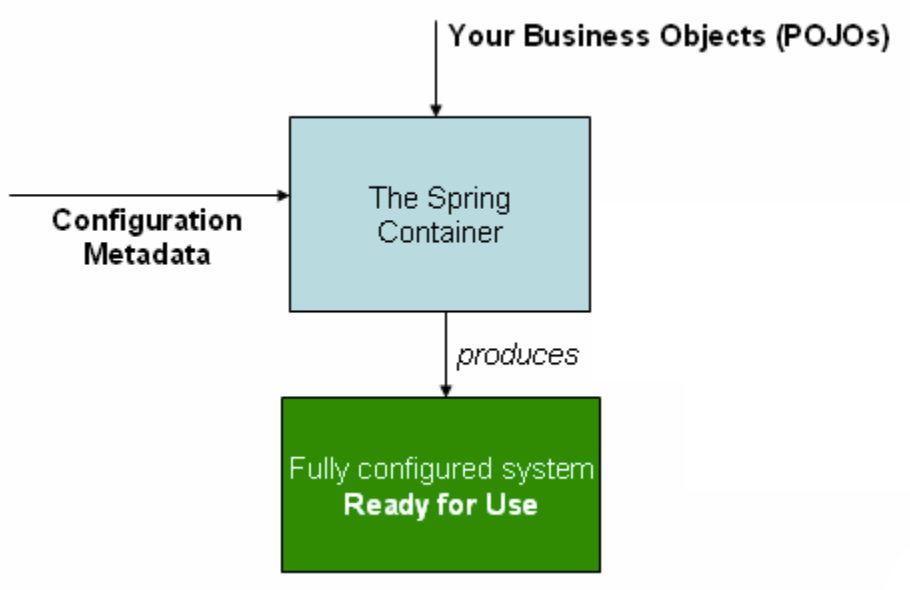
\includegraphics[width=0.6\linewidth]{./Figure/IMG_process.png}
    \caption{Spring IoC 容器}\label{Fig:xd1}
  \end{figure}

\subsection{配置元数据}
如上图所示,Spring IoC容器使用某种形式的配置元数据。 
此配置元数据表示应用程序开发人员如何告诉Spring容器实例化,配置和组装应用程序中的对象。

大多情况下,配置元数据以简单直观的XML格式提供,
因此本章大部分内容用XML格式的配置元数据来介绍Spring IoC容器的关键概念和功能。

\textbf{基于XML的元数据不是配置元数据的唯一允许形式。 Spring IoC容器本身与配置元数据的格式是完全脱钩。 如今,许多开发人员选择基于Java的配置来开发Spring应用程序。}

有关在Spring容器中其他形式的元数据的使用,请参见:

\begin{itemize}
    \item 基于注解的配置:Spring 2.5引入了对基于注解的配置元数据的支持。
    \item 基于Java的配置:从Spring 3.0开始,
    Spring JavaConfig项目提供的许多功能成为核心Spring Framework的一部分。 
    因此,可以使用Java而不是XML文件来定义应用程序类外部的bean。
     要使用这些新功能,请参见@ Configuration,@ Bean,@ Import和@DependsOn注解。
\end{itemize}

Spring配置由至少一个(通常是一个以上)容器管理的bean定义组成。 
基于XML的配置元数据将这些bean配置为顶级<beans/>元素内的<bean/>元素。
Java配置通常在@Configuration类中使用@Bean注释的方法。

这些bean定义对应于组成应用程序的实际对象。
通常,开发者定义服务层对象、数据访问对象(DAO)、表示对象(例如Struts Action实例)、基础结构对象(例如Hibernate SessionFactories,JMS队列)等等。
通常,开发者不会在容器中配置细粒度的域对象,因为DAO和业务逻辑通常负责它们的创建和加载。
但是,可以使用Spring与AspectJ的集成来配置在IoC容器的控制范围之外创建的对象。
请参阅使用AspectJ与Spring依赖注入域对象。

\newpage
以下示例显示了基于XML的配置元数据的基本结构:

\begin{figure}[ht]
    \centering
    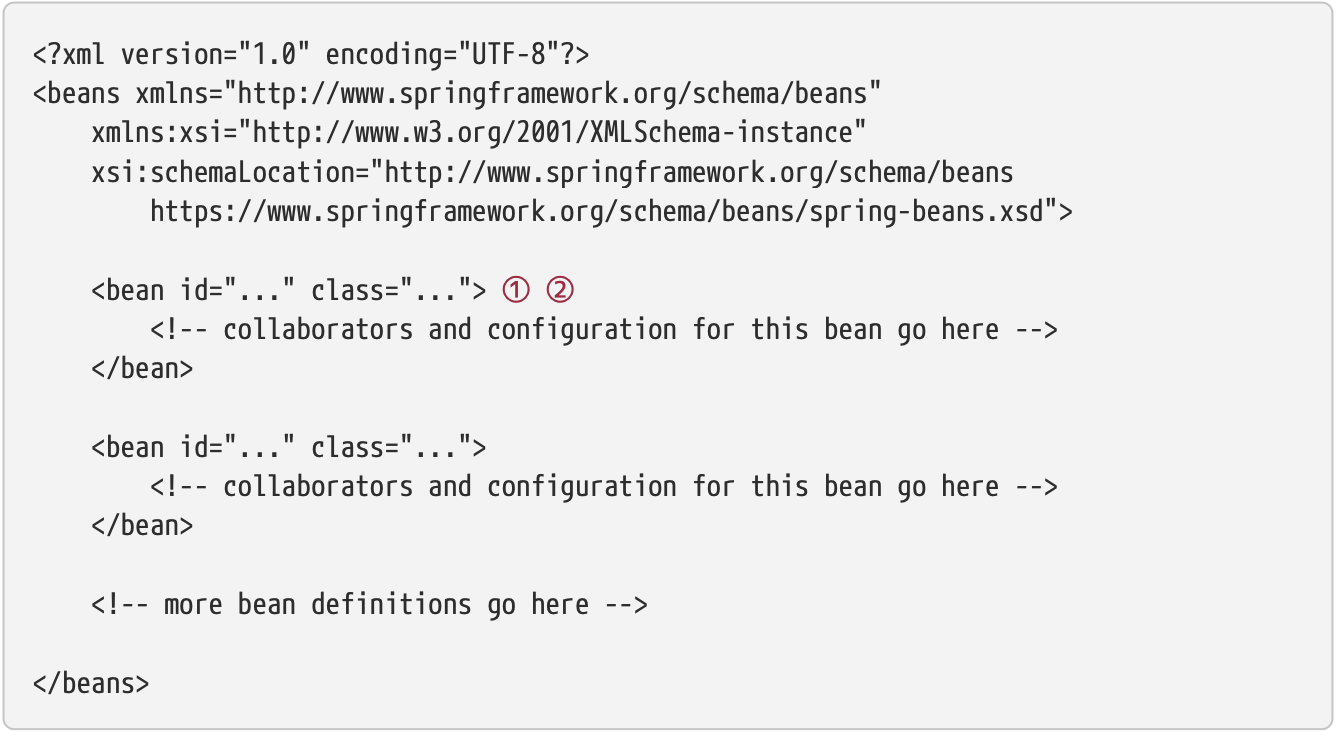
\includegraphics[width=1\linewidth]{./Figure/IMG_code_1.png}
  \end{figure}

\begin{enumerate}
    \item id属性是一个标识单个bean定义的字符串。
    \item class属性定义bean的类型,并使用完全限定的类名。
\end{enumerate}

id属性的值可以作为对象引用,并在其他bean 定义中被引用。 
在此示例中未描述如何进行对象引用。 有关更多信息,请参见依赖项。

\subsection{实例化容器}
ApplicationContext构造函数的参数是表示资源位置路径的字符串,
这些资源字符串使容器可以从各种外部资源(例如本地文件系统,Java CLASSPATH等)加载配置元数据。

\begin{figure}[ht]
\centering
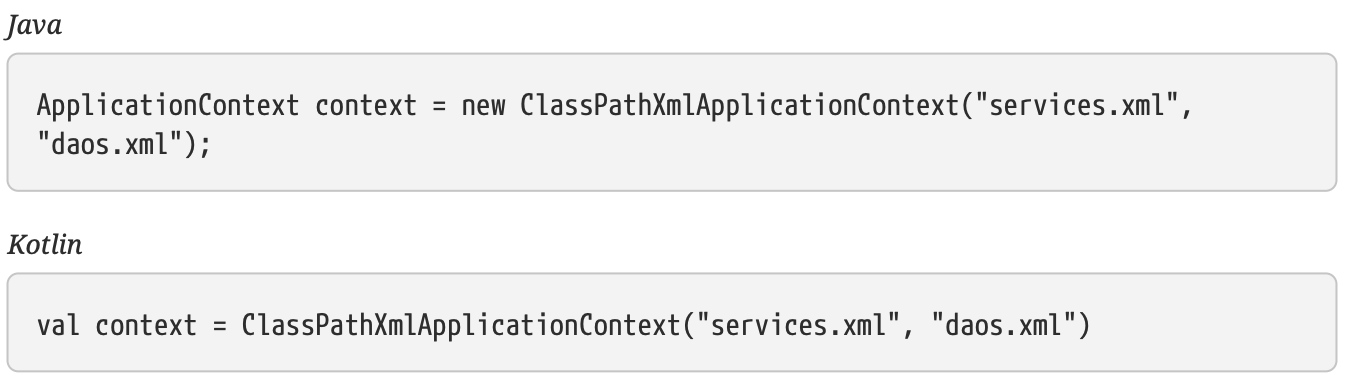
\includegraphics[width=1\linewidth]{./Figure/IMG_code_2.png}
\end{figure}

\newpage

\textbf{在了解了Spring的IoC容器之后,您可能想了解更多有关Spring的Resource抽象(如参考资料所述),它提供了一种从URI语法中定义的位置读取InputStream的机制。 尤其是在应用程序上下文和资源路径中所述,资源路径用于构造应用程序上下文。}

以下示例显示了服务层对象(services.xml)的配置文件:

\begin{figure}[ht]
\centering
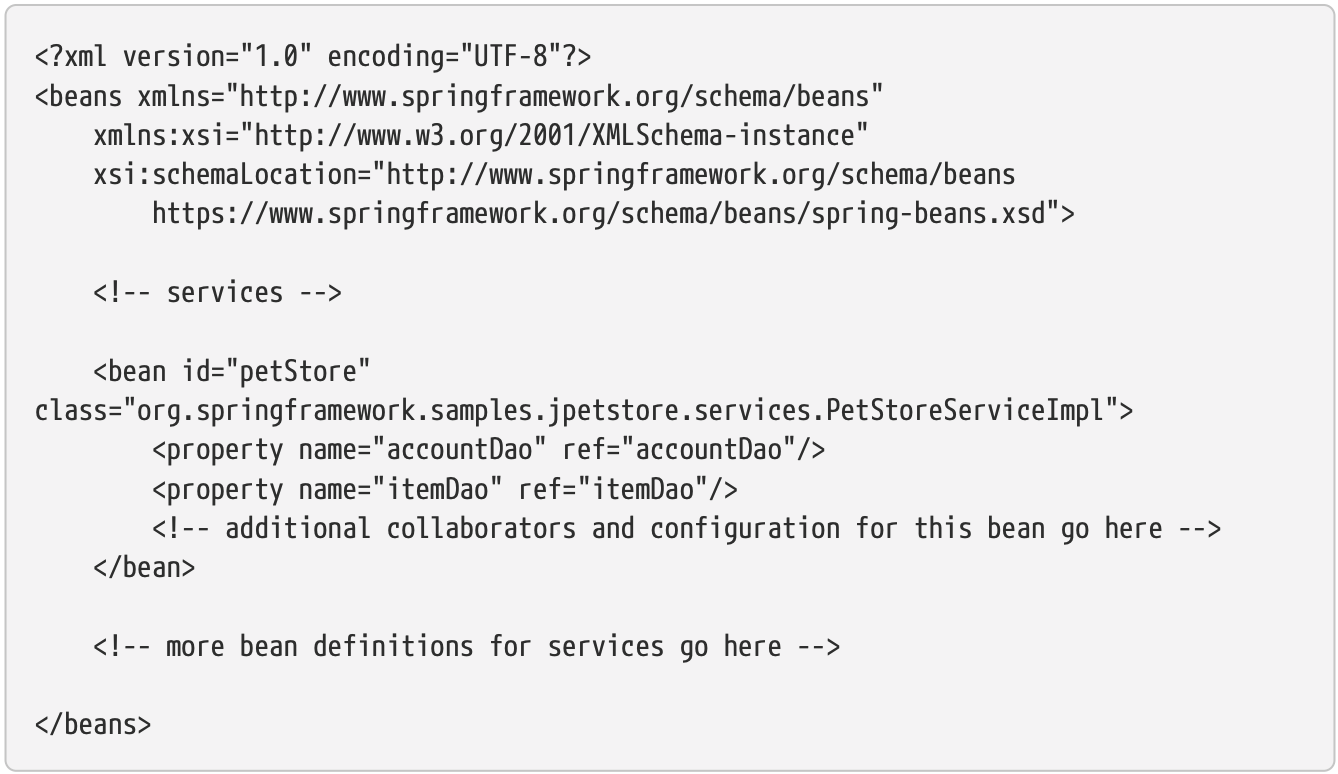
\includegraphics[width=1\linewidth]{./Figure/IMG_code_3.png}
\end{figure}

以下示例显示了数据访问对象(daos.xml)文件:

\begin{figure}[ht]
\centering
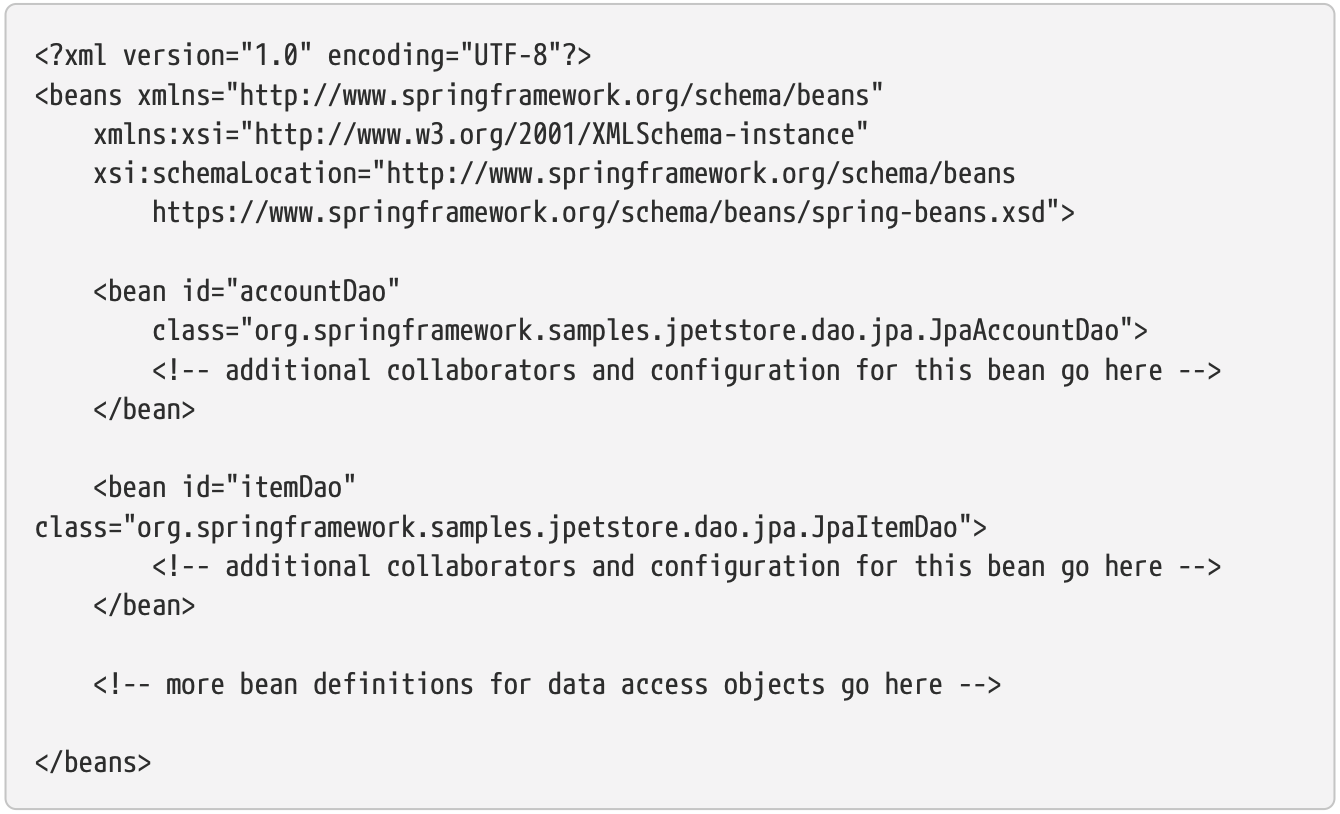
\includegraphics[width=1\linewidth]{./Figure/IMG_code_4.png}
\end{figure}

在前面的示例中,服务层由PetStoreServiceImpl类和两个JpaAccountDao
和JpaItemDao类型的数据访问对象组成(基于JPA对象关系映射标准)。
 属性名称元素引用JavaBean属性的名称,而ref元素引用另一个bean定义的名称。 
 id和ref元素之间的这种联系表达了协作对象之间的依赖性。 
 有关配置对象的依存关系的详细信息,请参阅依存关系。

 \subsubsection{组合基于XML的配置元数据}
 使bean定义跨越多个XML文件可能会很有用。 
 通常,每个单独的XML配置文件都代表体系结构中的逻辑层或模块。

 您可以使用应用程序上下文构造函数从所有这些XML片段中加载bean定义。 
 如上一节中所示,此构造函数具有多个Resource位置。
  或者,使用一个或多个出现的<import/>元素从另一个文件中加载bean定义。 
  以下示例显示了如何执行此操作:

  \begin{figure}[ht]
    \centering
    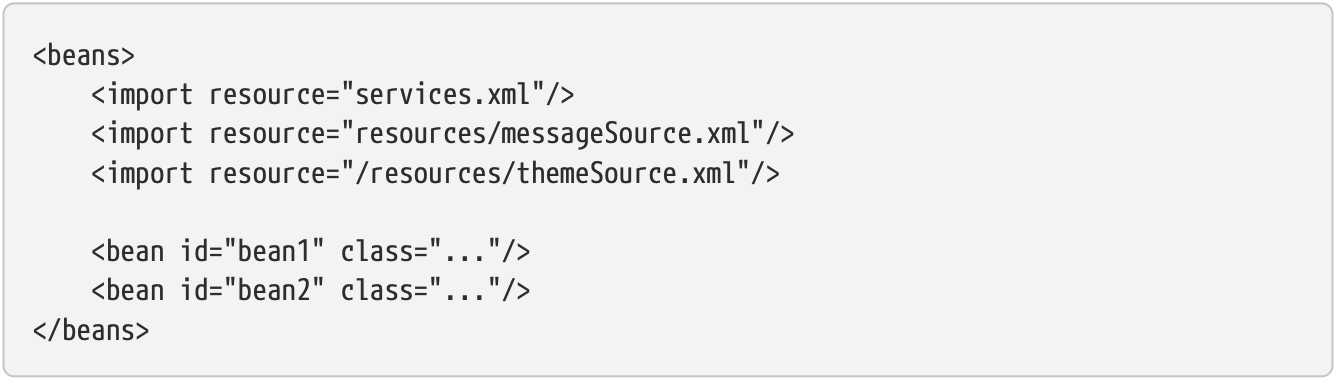
\includegraphics[width=1\linewidth]{./Figure/IMG_code_5.png}
    \end{figure}

    在前面的示例中,外部bean定义是从以下三个文件加载的:services.xml,messageSource.xml和themeSource.xml。 
    所有位置路径都相对于进行导入的定义文件,因此,services.xml必须与进行导入的文件位于同一目录或类路径位置,
    而messageSource.xml和themeSource.xml必须位于进行导入的文件的位置下方的资源位置。 
    因此,斜杠被忽略。 但是,鉴于这些路径是相对的,最好不要使用任何斜线。 
    根据Spring Schema,导入的文件的内容(包括顶级<beans />元素)必须是有效的XML bean定义。

\textbf{可以但不建议使用相对的“ ../”路径引用父目录中的文件。 这样做会创建对当前应用程序外部文件的依赖关系。 特别是,不建议使用classpath:URL(例如,classpath:../ services.xml),在运行时的解析过程会选择“最近”的classpath根目录,然后查看其父目录。 类路径配置的更改可能会导致选择其他错误的目录。}

\textbf{您始终可以使用完全限定的资源位置来代替相对路径:例如,file:C:/config/ser-vices.xml或classpath:/config/services.xml。 但是请注意,您正在将应用程序的配置耦合到特定的绝对位置。 通常,最好为这样的绝对位置保留一个间接寻址。例如,通过在运行时针对JVM系统属性解析的“ \$ \{…\}”占位符。}

    命名空间本身提供了导入指令功能。 
    Spring中的一系列XML名称空间(例如,上下文和util名称空间)
    提供了超出普通bean定义的其他配置功能。

\subsubsection{Groovy Bean定义DSL}
作为外部化配置元数据的另一个示例,
Bean定义也可以在Spring的Groovy Bean定义DSL中表达,
类似Grails。 
通常,这种配置位于“.groovy”文件中,其结构如以下示例所示:

\begin{figure}[ht]
    \centering
    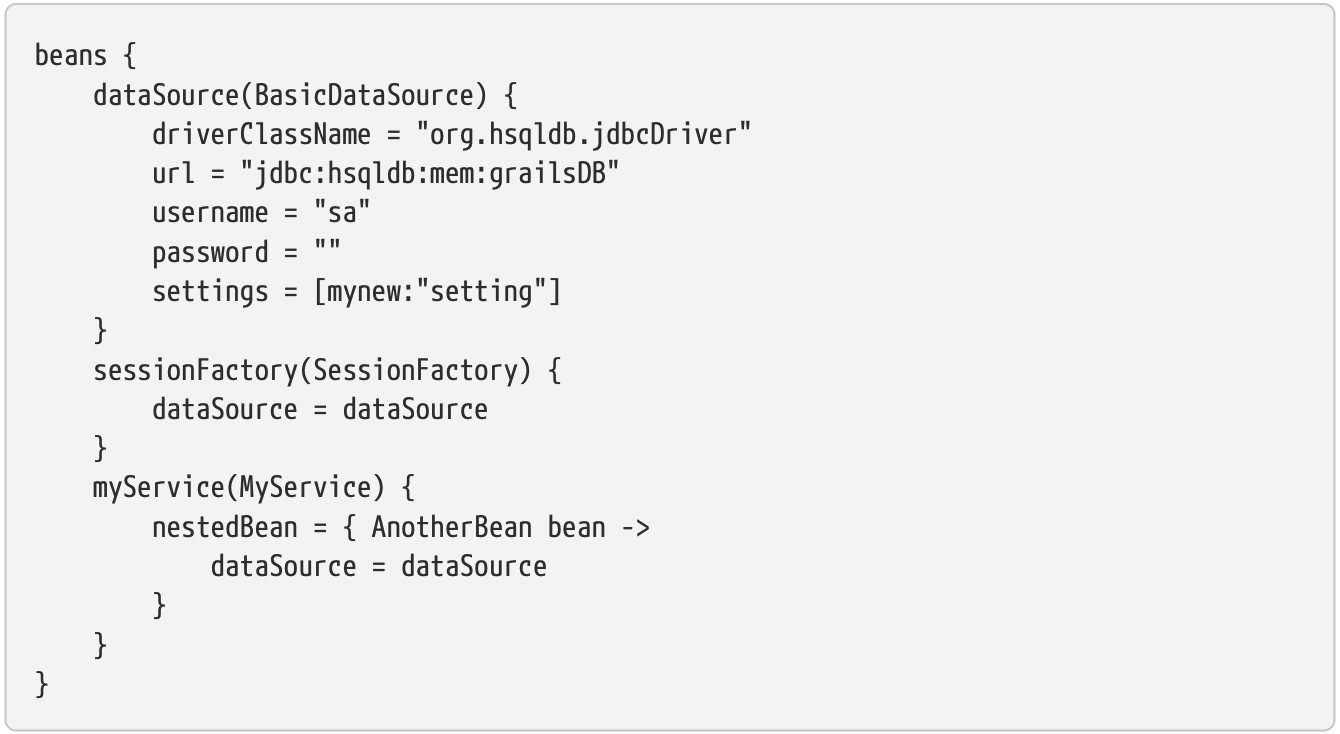
\includegraphics[width=1\linewidth]{./Figure/IMG_code_6.png}
\end{figure}
    
这种配置样式在很大程度上等同于XML Bean定义,甚至支持Spring的XML配置名称空间。 
它还允许通过importBeans指令导入XML bean定义文件。

\subsection{使用容器}

ApplicationContext是高级工厂的接口,
该工厂能够维护不同bean及其依赖关系的注册表。 
通过使用方法T getBean(String name,Class <T> requiredType),可以检索bean的实例。

ApplicationContext允许您读取bean定义并访问它们,如以下示例所示:

\begin{figure}[ht]
    \centering
    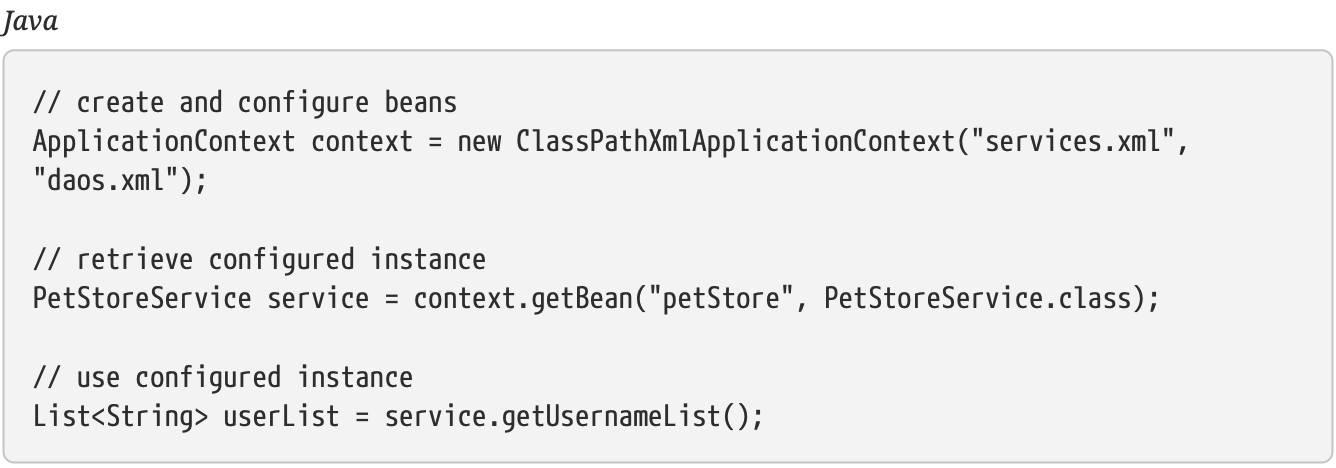
\includegraphics[width=1\linewidth]{./Figure/IMG_code_7.png}
\end{figure}

\newpage
\begin{figure}[ht]
    \centering
    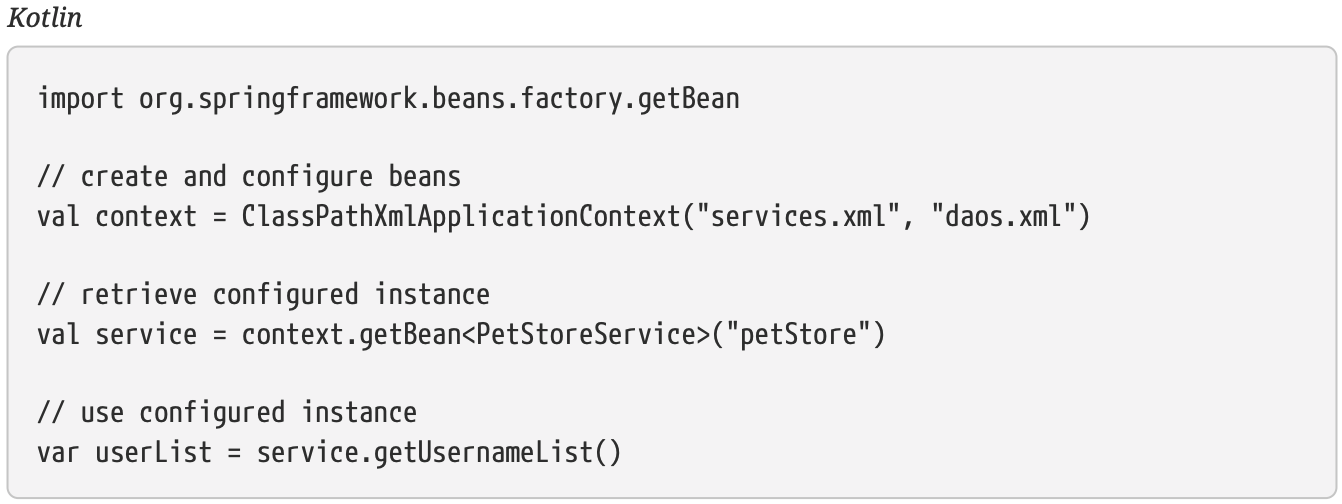
\includegraphics[width=1\linewidth]{./Figure/IMG_code_8.png}
\end{figure}

使用Groovy配置也非常相似。 
它有一个不同的上下文实现类,该类可以识别Groovy(但也可以解析XML Bean定义)。
 以下示例显示了Groovy配置:

 \begin{figure}[ht]
    \centering
    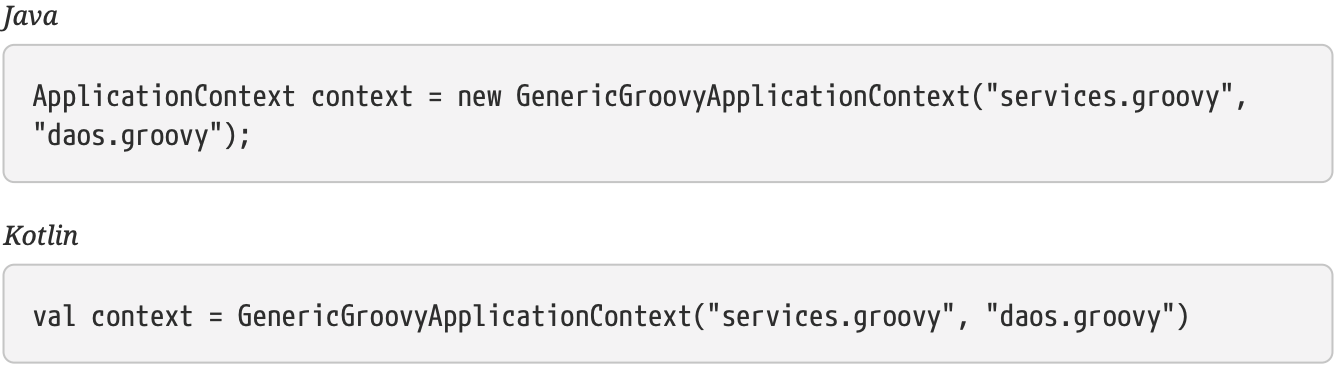
\includegraphics[width=1\linewidth]{./Figure/IMG_code_9.png}
\end{figure}

\newpage
最灵活的变体是将GenericApplicationContext与读取委托器结合在一起,例如,与用于XML文件的XmlBeanDefinitionReader结合使用,如以下示例所示:

\begin{figure}[ht]
    \centering
    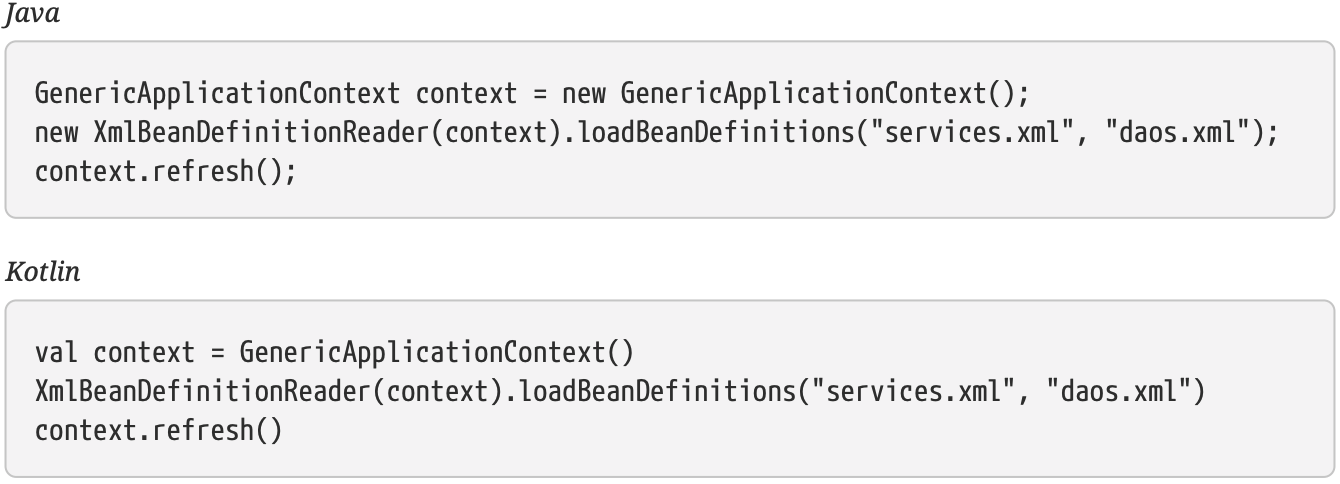
\includegraphics[width=1\linewidth]{./Figure/IMG_code_10.png}
\end{figure}

类似的,还可以将GroovyBeanDefinitionReader用于Groovy文件,如以下示例所示:

\begin{figure}[ht]
    \centering
    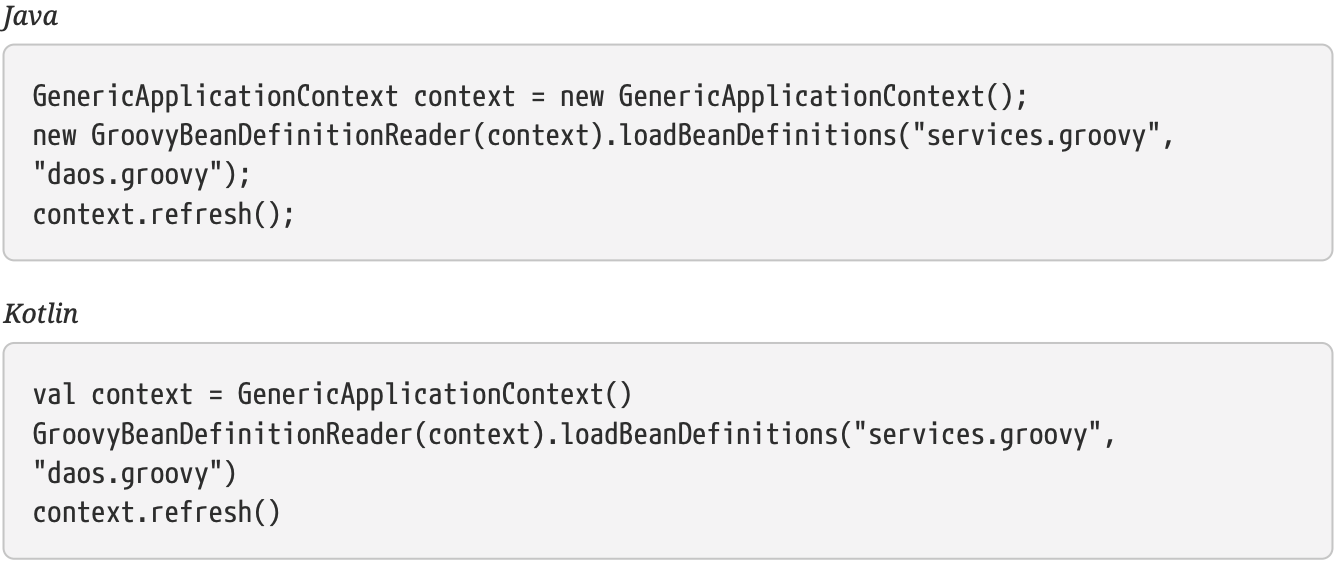
\includegraphics[width=1\linewidth]{./Figure/IMG_code_11.png}
\end{figure}

开发者可以在同一ApplicationContext上混用不用的阅读委托器来从不同的配置源读取Bean定义。

然后,可以使用getBean检索bean的实例。 
ApplicationContext接口还有其他几种检索bean的方法,
但是理想情况下,永远不要使用它们。 
实际上,您的应用程序代码应该根本不调用getBean()方法,完全不依赖于Spring API。 
例如,Spring与Web框架的集成为各种Web框架组件(如控制器和JSF托管的bean)提供了依赖注入,
开发者可以通过元数据(例如自动装配注释)声明对特定bean的依赖。

\section{Bean概述}
Spring IoC容器管理一个或多个bean。 
这些bean是使用开发者提供给容器的配置元数据创建的(例如,以XML <bean/>定义的形式)。 
在容器本身内,这些bean定义表示为BeanDefinition对象,其中包含(除其他信息外)以下元数据:

\begin{itemize}
    \item 包限定的类名:定义了Bean的实际实现类。
    \item Bean行为配置元素,用于声明Bean在容器中的行为(作用域,生命周期回调等)。
    \item 引用其他bean来完成其工作所需要的。 这些引用也称为协作者或依赖项。
    \item 要在新创建的对象中设置的其他配置设置-例如,池的大小限制或要在管理连接池的bean中使用的连接数。
\end{itemize}

此元数据转换为构成每个bean定义的一组属性。 下表描述了这些属性:

\begin{longtable}[ht]{|l|l|}
    \caption{Bean 定义}\\
    \hline
    属性&解释于...\\
    \hline
    类&Bean实例化\\
    \hline
    名称&Bean命名\\
    \hline
    范围&Bean作用范围\\
    \hline
    构造函数参数&依赖注入\\
    \hline
    参数&依赖注入\\
    \hline
    自动装配模式&自动装配依赖\\
    \hline
    懒加载模式&懒加载Bean\\
    \hline
    初始化方法&初始化回调\\
    \hline
    销毁方法&销毁回调\\
    \hline
\end{longtable}

除了包含有关如何创建特定bean的信息的bean定义之外,
ApplicationContext实现还允许注册在容器外部(由用户)创建的现有对象。
这是通过通过getBeanFactory()方法访问ApplicationContext的BeanFactory来完成的
,该方法返回BeanFactory DefaultListableBeanFactory实现。
DefaultListableBeanFactory通过registerSingleton(..)和registerBeanDefinition(..)
方法支持此注册。 但是,典型的应用程序只能与通过常规bean定义元数据定义的bean一起使用。

\textbf{Bean元数据和手动提供的单例实例需要尽早注册,以便容器在自动装配和其他自省步骤中正确地推理它们。 虽然在某种程度上支持覆盖现有元数据和现有单例实例,但是在运行时(与对工厂的实时访问同时)对新bean的注册不被正式支持,并且可能导致并发访问异常或导致bean容器中的状态不一致。}

\subsection{Bean命名}

每个bean具有一个或多个标识符。 这些标识符在承载Bean的容器内必须是唯一的。 
一个bean通常只有一个标识符。 
但是,如果有多个,则将其余的视为别名。

在基于XML的配置元数据中,可以使用id属性和name属性来指定bean标识符。
id属性可以精确指定一个id。 
通常,这些名称是字母数字(“ myBean”,“ someService”等),
但它们也可以包含特殊字符。 如果要为bean引入其他别名,
还可以在name属性中指定它们,并用逗号,分号或空格分隔。 
在Spring 3.1之前的版本中,id属性定义为xsd:ID类型,该类型限制了可能的字符。
从3.1开始,它被定义为xsd:string类型。 
但是,bean ID唯一性仍由容器强制执行,尽管不再由XML解析器执行。

开发者不需要提供Bean的名称或ID。 
如果未明确提供名称或ID,则容器将为该bean生成一个唯一的名称。 
但是,如果要通过使用ref元素或服务定位器样式引用该bean,则必须提供一个名称。
不提供名称一般在使用内部bean和自动装配依赖情况下存在。

\begin{center}
    \textbf{Bean命名约定}
\end{center}

\textit{约定即在命名bean时使用标准Java字段命名规范。 也就是说,bean名称以小写字母开头,并用驼峰式大小写。 此类名称的示例包括accountManager,accountService,userDao,loginController等。}

\textit{一致地命名Bean使您的配置更易于阅读和理解。 另外,如果您使用Spring AOP,则在将增强应用于名称相关的一组bean时,它会很有帮助。}

\textbf{通过在类路径中进行组件扫描,Spring会按照前面描述的规则为未命名的组件生成Bean名称:从本质上讲,采用简单的类名称并将其初始字符转换为小写。 但是,在(不寻常的)特殊情况下,如果有多个字符并且第一个和第二个字符均为大写字母,则会保留原始大小写。 这些规则与java.beans.Introspector.decapitalize(Spring在此使用)定义的规则相同。}

\subsubsection{在Bean定义之外定义Bean的别名}
在bean定义中,可以使用id属性和name实现来定义多个bean名称。
这些名称可以是同一个bean的等效别名,并且在某些情况下很有用,
例如通过使用特定于该组件本身的bean名称,让应用程序中的每个组件都引用一个公共依赖项。

但是,在实际定义bean的地方指定所有别名并不总是足够的。 
有时需要为在别处定义的bean引入别名。 
在大型系统中,配置定义在每个子系统中,每个子系统都有自己的对象定义集。 
在基于XML的配置元数据中,可以使用<alias />元素来完成此操作。 
以下示例显示了如何执行此操作:

\begin{figure}[ht]
    \centering
    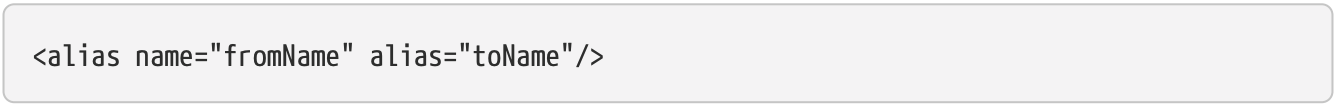
\includegraphics[width=1\linewidth]{./Figure/IMG_code_12.png}
\end{figure}
在上面的例子中,
在使用该别名定义之后,
名为fromName的bean(在同一容器中)也就是toName。

例如,子系统A的配置元数据可以通过subsystemA-dataSource的名称引用数据源。 
子系统B的配置元数据可以通过subsystemB-dataSource的名称引用数据源。 
组成使用这两个子系统的主应用程序时,主应用程序通过myApp-dataSource的名称引用数据源。
要使所有三个名称都引用相同的对象,可以将以下别名定义添加到配置元数据中:

\begin{figure}[ht]
    \centering
    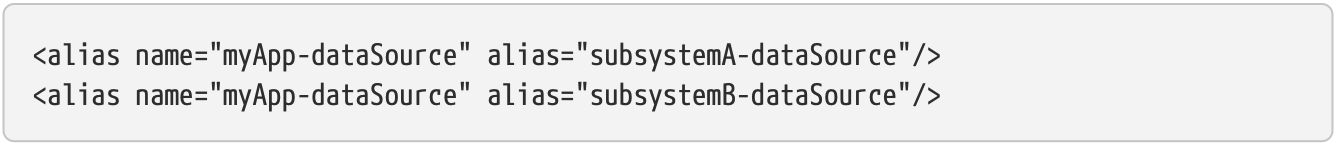
\includegraphics[width=1\linewidth]{./Figure/IMG_code_13.png}
\end{figure}

现在,每个组件和主应用程序都可以通过唯一的名称引用数据源,并保证不会与任何其他定义冲突(有效地创建名称空间),但是它们引用的是同一bean。

\begin{center}
    \textbf{Java配置}
\end{center}

\textit{如果使用Java configuration,则@Bean注解可用于提供别名。 有关详细信息,请参见使用@Bean批注。}

\subsection{Bean 实例化}
Bean定义本质上是创建一个或多个对象的基础数据。 
当bean被需要时,容器将查找对应的bean定义,
并使用该bean定义封装的配置元数据来创建(或获取)实际对象。

如果使用基于XML的配置元数据,则在<bean />元素的class属性中指定要实例化的对象的类型(或类)。 
这个class属性(在内部是BeanDefinition实例的Class属性)通常是必需的。 
(有关异常,请参阅使用实例工厂方法实例化和Bean定义继承。)
可以通过以下两种方式之一使用Class属性:

\begin{itemize}
    \item 通常,指定要构造的Bean类,在容器本身通过反射性地调用其构造函数直接创建Bean的情况下,这在某种程度上等同于使用new运算符的Java代码。
    \item 要指定包含用于创建对象的静态工厂方法的实际类,在不太常见的情况下,容器将在类上调用静态工厂方法以创建Bean。 从静态工厂方法的调用返回的对象类型可以是同一类,也可以是完全不同的另一类。
\end{itemize}

\begin{center}
    \textbf{嵌套的类名}
\end{center}

\textit{如果要为嵌套类配置Bean定义,则可以使用嵌套类的二进制名称或源名称。}

\textit{例如,如果com.example包中有一个名为SomeThing的类,并且此SomeThing类具有一个名为OtherThing的静态嵌套类,则可以用美元符号(\$)或点(。)分隔。 因此,bean定义中class属性的值将为com.example.SomeThing \$ OtherThing或com.example.SomeThing.OtherThing。}

\subsubsection{使用构造函数实例化}
当通过构造函数方法创建bean时,所有普通类都可以被Spring使用并与之兼容。 
也就是说,正在开发的类不需要实现任何特定的接口或以特定的方式进行编码。 
只需指定bean类就足够了。 但是可能需要一个默认(空)构造函数。

Spring IoC容器几乎可以管理任何类,不仅限于管理真正的JavaBean。 
大多数Spring用户更喜欢实际的JavaBean,
它仅具有默认(无参数)构造函数,并具有根据容器中的属性建模的适当的setter和getter。 
还可以在容器中拥有更多奇特的非Bean风格的类,例如,如果需要使用绝对不符合JavaBean规范的旧式连接池,
Spring也可以对其进行管理。

使用基于XML的配置元数据,可以如下指定bean类:

\begin{figure}[ht]
    \centering
    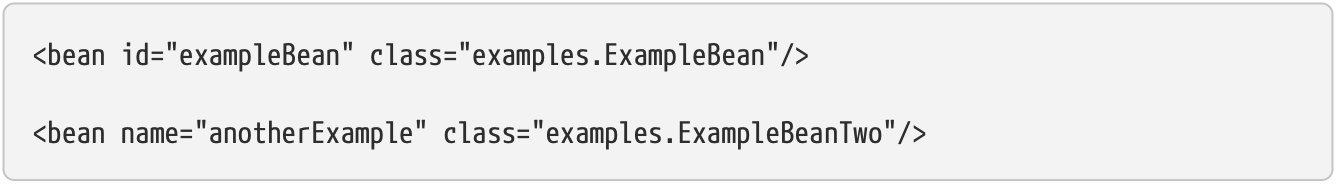
\includegraphics[width=1\linewidth]{./Figure/IMG_code_14.png}
\end{figure}

有关向构造函数提供参数(如果需要)并在构造对象之后设置对象实例属性的机制的详细信息,请参见\textbf{依赖注入}。

\subsubsection{使用静态工厂方法实例化}
定义使用静态工厂方法创建的bean时,请使用class属性指定包含静态工厂方法的类,
并使用名为factory-method的属性指定工厂方法本身的名称。 
程序应该能够调用此方法(后面解释带有可选参数的情况),并返回一个活动对象,
该对象随后将被视为已通过构造函数创建。 
这种bean定义的一种用法是在旧版代码中调用静态工厂。

以下bean定义指定通过调用工厂方法来创建bean。 
这种定义不能指定返回对象的类型(类),仅能指定包含工厂方法的类。  以下示例显示如何指定工厂方法,
在此示例中,createInstance()方法必须是静态方法:

\begin{figure}[ht]
    \centering
    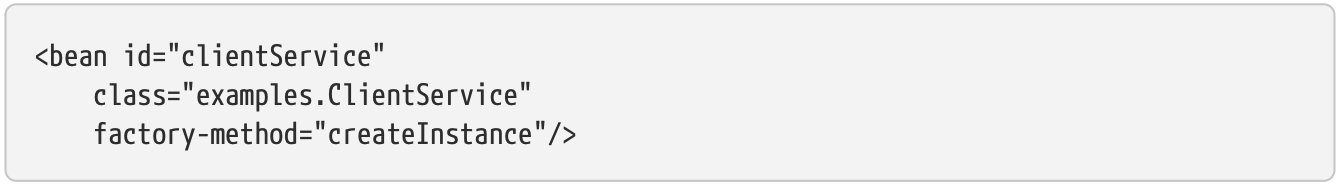
\includegraphics[width=1\linewidth]{./Figure/IMG_code_15.png}
\end{figure}

\newpage
以下示例显示了需要与前面的bean定义一起使用的类:

\begin{figure}[ht]
    \centering
    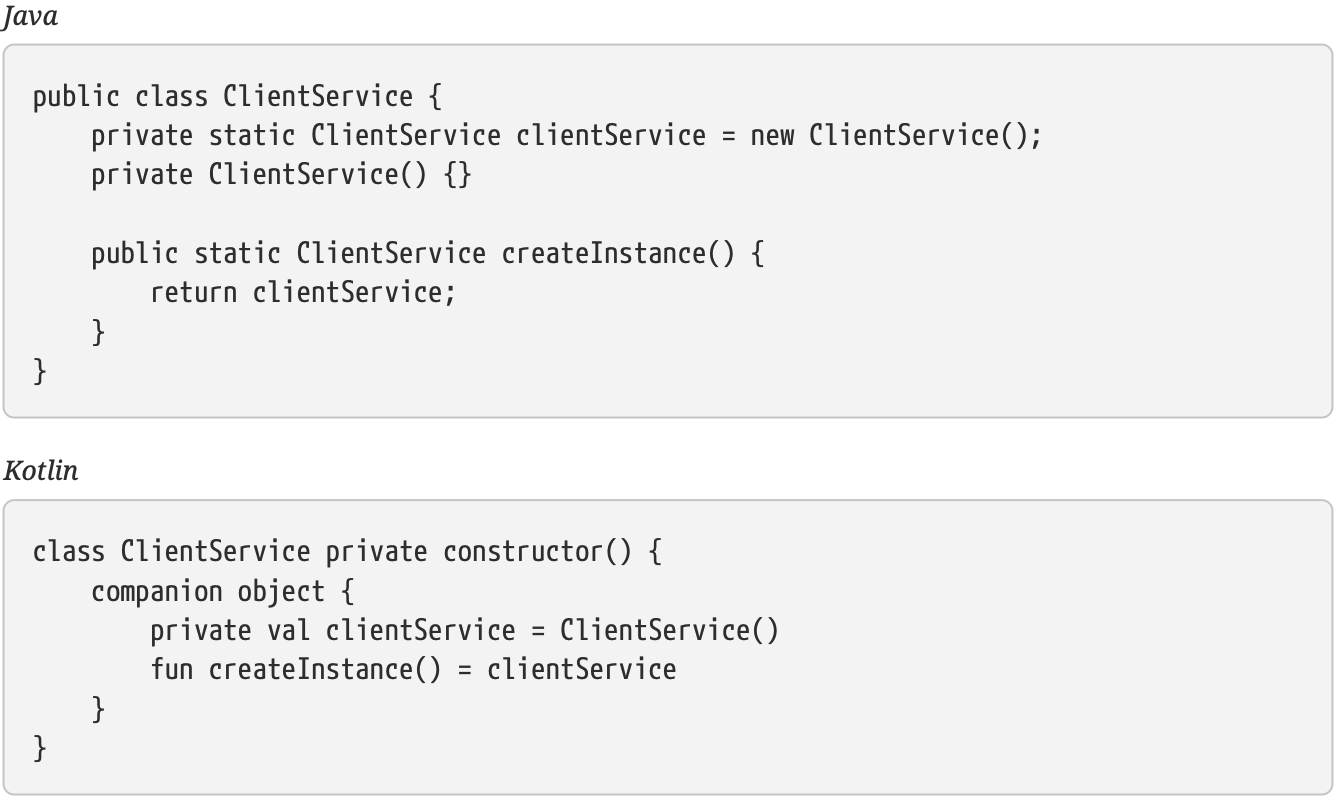
\includegraphics[width=1\linewidth]{./Figure/IMG_code_16.png}
\end{figure}

有关为工厂方法提供(可选)参数并在从工厂返回对象后设置对象实例属性的机制的详细信息,
请参阅详细信息中的依赖关系和配置。

\subsubsection{使用实例工厂方法实例化}
类似于通过静态工厂方法进行实例化,
使用实例工厂方法进行实例化会从容器中调用现有bean的非静态方法来创建新bean。 
要使用此机制,请将class属性保留为空,并在factory-bean属性中,
在当前(或父或祖先)容器中指定包含要创建该对象的实例方法的Bean的名称。 
使用factory-method属性设置工厂方法本身的名称。 以下示例显示了如何配置此类Bean:

\begin{figure}[ht]
    \centering
    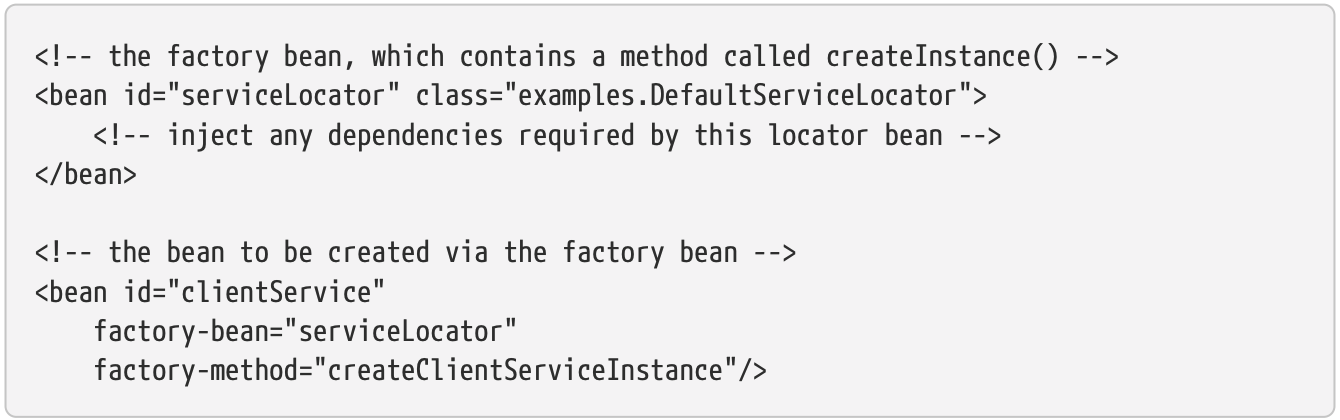
\includegraphics[width=1\linewidth]{./Figure/IMG_code_17.png}
\end{figure}

以下示例显示了相应的类:

\begin{figure}[ht]
    \centering
    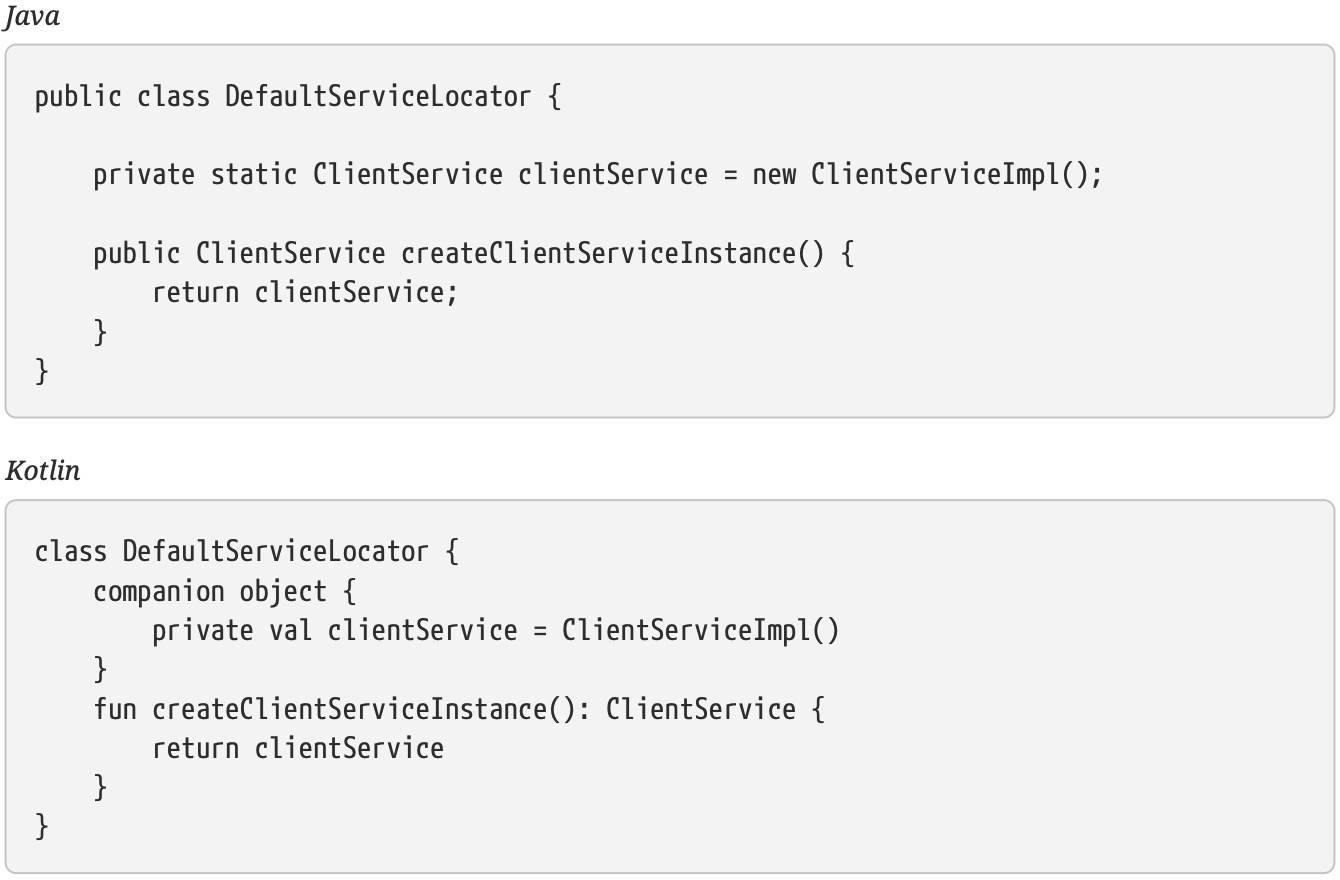
\includegraphics[width=1\linewidth]{./Figure/IMG_code_18.png}
\end{figure}

\newpage
一个工厂类也可以包含一个以上的工厂方法,如以下示例所示:

\begin{figure}[ht]
    \centering
    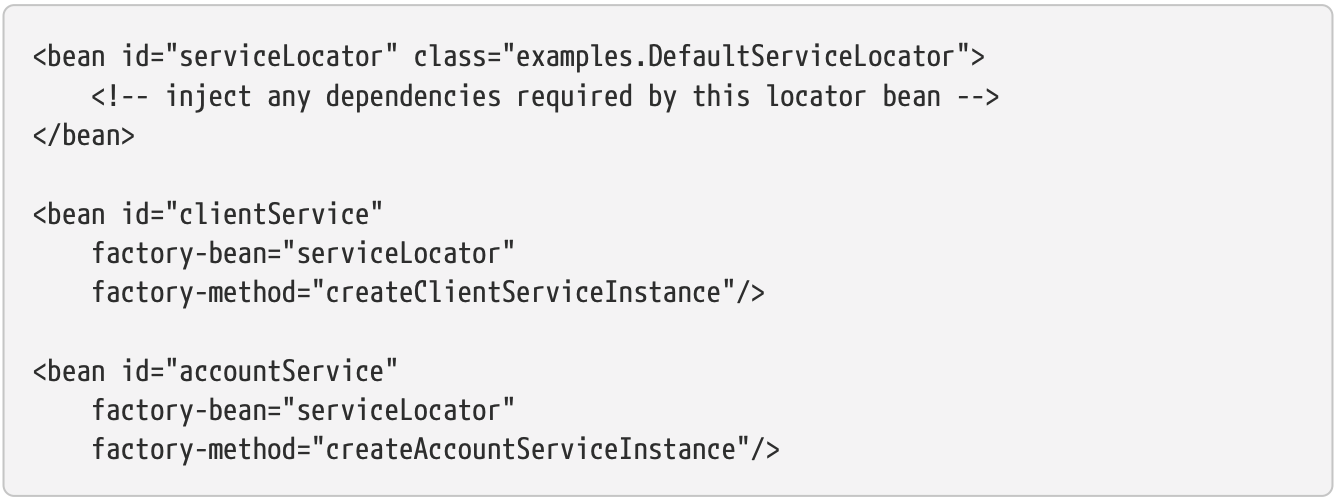
\includegraphics[width=1\linewidth]{./Figure/IMG_code_19.png}
\end{figure}

\newpage
以下示例显示了相应的类:
\begin{figure}[ht]
    \centering
    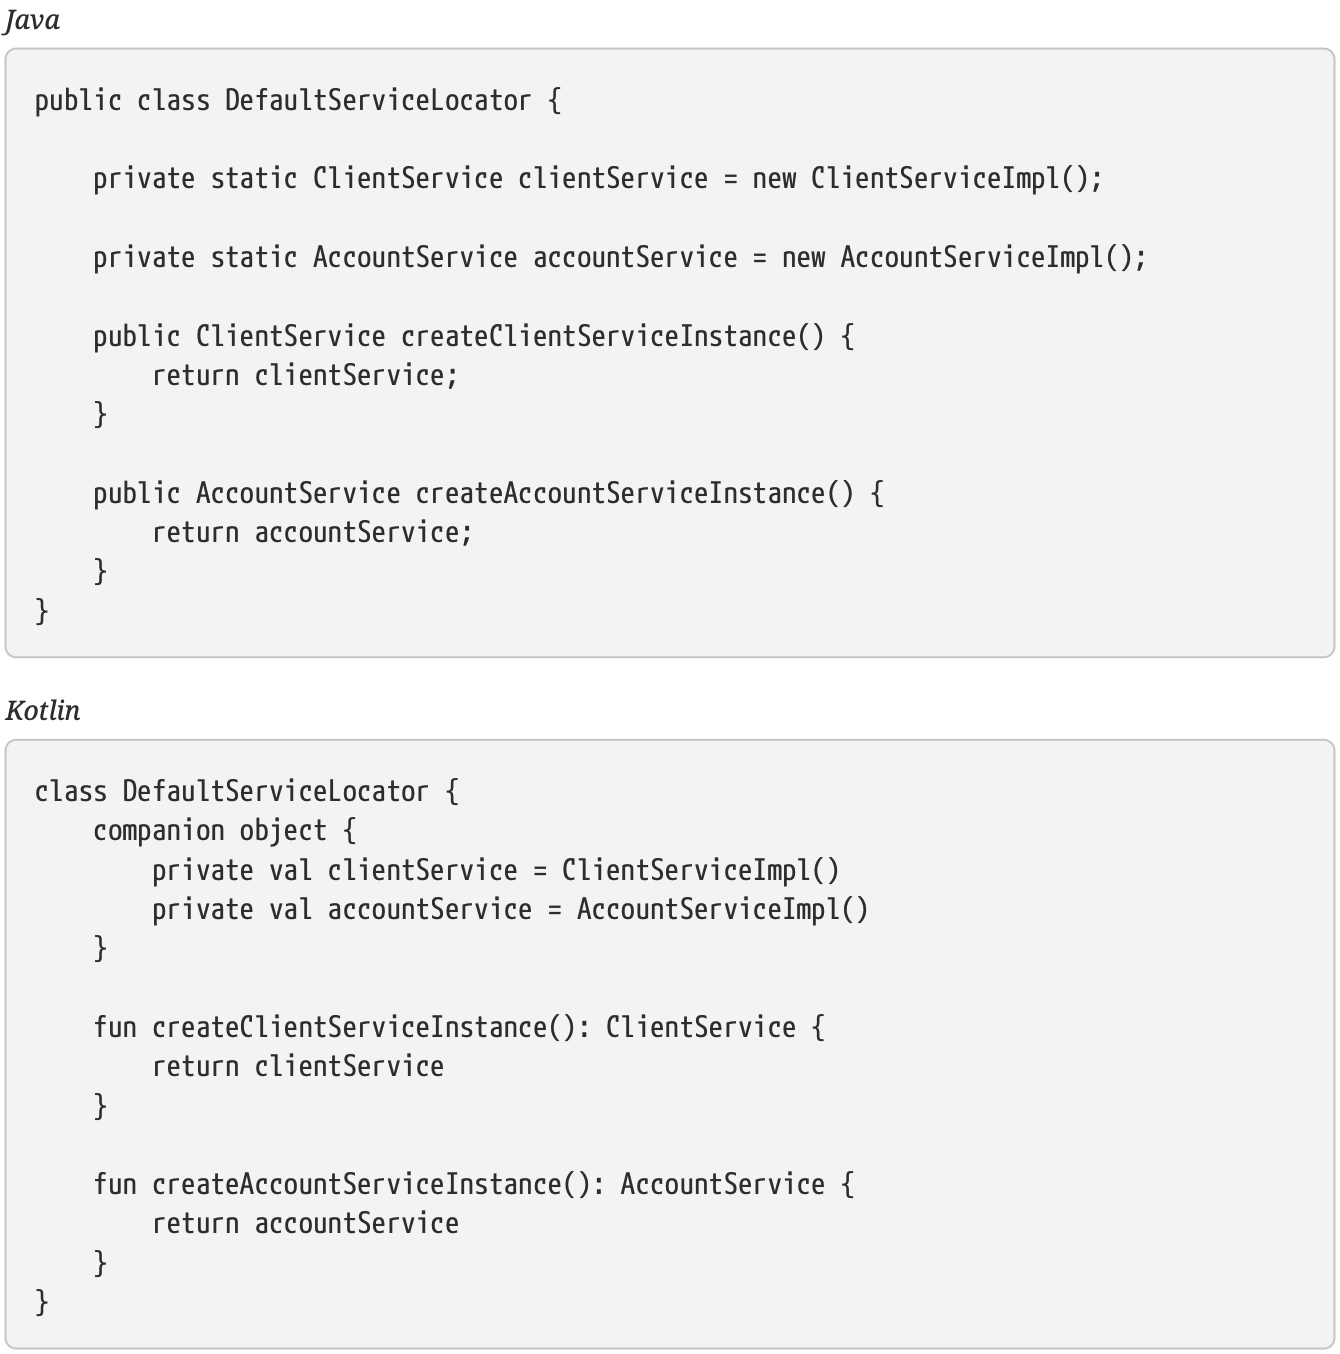
\includegraphics[width=1\linewidth]{./Figure/IMG_code_20.png}
\end{figure}

这种方法表明,工厂Bean本身可以通过依赖项注入(DI)进行管理和配置。 
详细信息,请参见依赖和配置。

\textbf{在Spring文档中,“ factory bean”是指在Spring容器中配置并通过实例或静态工厂方法创建对象的bean。 相比之下,FactoryBean(请注意大小写)是指特定于Spring的FactoryBean实现类。}

\subsubsection{确定Bean的运行时类型}
确定特定bean的运行时类型并非易事。
 Bean元数据定义中的指定类只是初始类引用,
 可能与声明的工厂方法结合使用,或者是FactoryBean类,
 这可能导致Bean的运行时类型不同,或者在实例工厂方法的情况下完全不进行设置(通过指定的factory-bean名称解析)。
此外,AOP代理可以使用基于接口的代理包装bean实例,
而目标Bean的实际类型(仅是其接口的实现类)的暴露程度有限。

找出特定bean的实际运行时类型的推荐方法是对指定bean名称的BeanFactory.getType调用。 
这考虑了上述所有情况,并返回了与BeanFactory.getBean相同的对象类型。

\section{依赖}
典型的企业应用程序不包含单个对象(或Spring术语中的bean)。 即使是最简单的应用程序,也有一些对象可以协同工作,以呈现最终用户视为一致的应用程序。 下一部分将说明如何从定义多个独立的bean定义到实现对象协作以实现目标的完全实现的应用程序。

\subsection{依赖注入}

依赖注入(DI)是一个过程,
通过该过程,对象只能通过构造函数参数,
工厂方法的参数或在构造或创建或从工厂方法返回对象实例后在对象实例上设置的属性来定义其依赖关系
(即,与它们一起工作的其他对象)。 然后,容器在创建bean时注入那些依赖项。 
此过程从根本上讲是通过使用类的直接构造或服务定位器模式来控
制其自身的实例化或位置的Bean本身的逆过程(因此称为控制反转)。

使用DI原理,代码更简洁,
当为对象提供依赖项时,去耦会更有效。 
该对象不查找其依赖项,并且不知道依赖项的位置或类。 
因此类变得更易于测试,尤其是当依赖项依赖于接口或抽象基类时,
它们允许在单元测试中使用存根或模拟实现。

DI存在两个主要变体:基于构造函数的依赖注入和基于Setter的依赖注入。

\subsubsection{基于构造函数的依赖注入}
基于构造函数的DI是通过容器调用具有多个参数(每个参数代表一个依赖项)的构造函数来完成的。 调用带有特定参数的静态工厂方法来构造Bean几乎是等效的,并且本次讨论将构造函数和静态工厂方法的参数视为类似。 以下示例显示了只能通过构造函数注入进行依赖项注入的类:

\begin{figure}[ht]
    \centering
    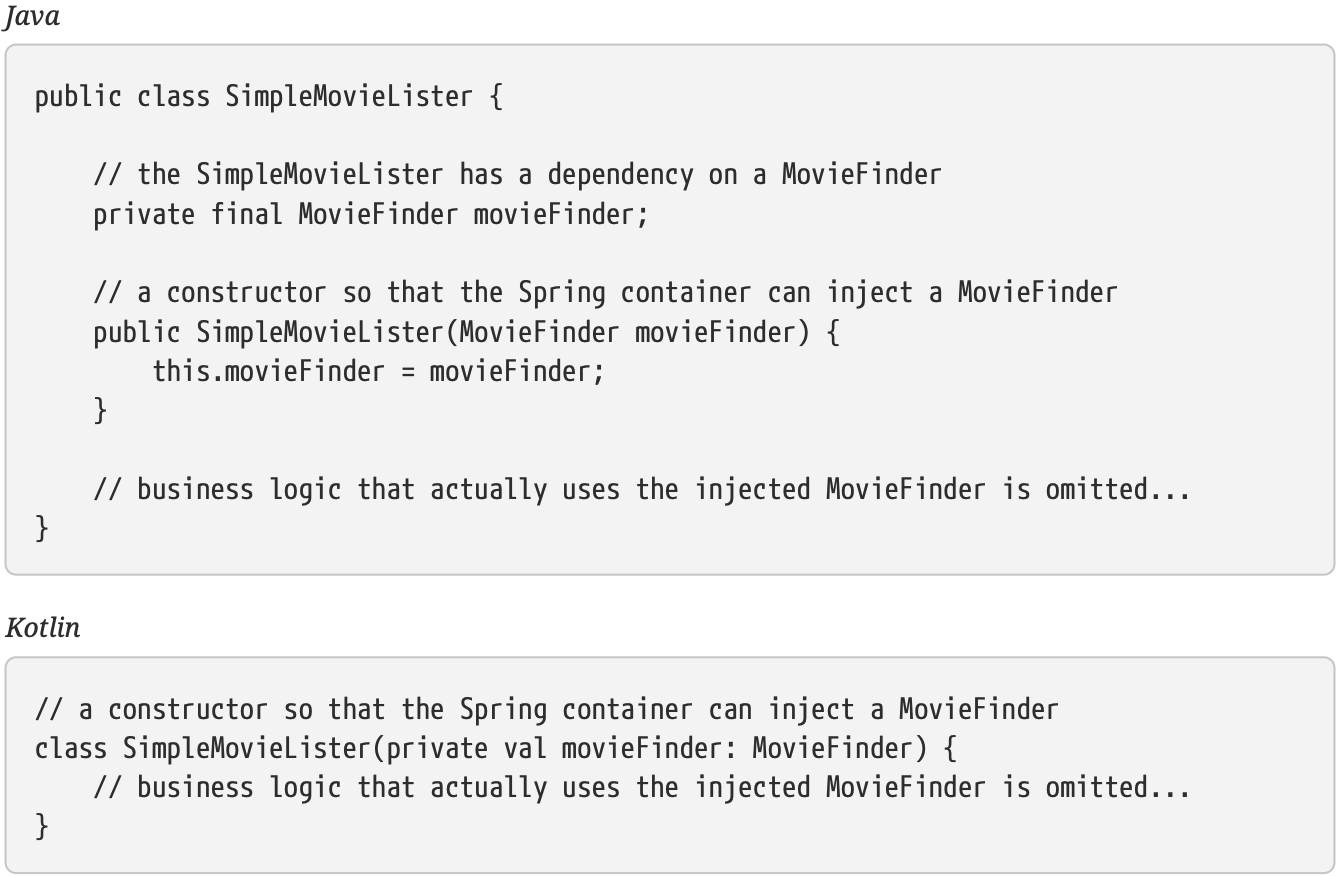
\includegraphics[width=1\linewidth]{./Figure/IMG_code_21.png}
\end{figure}

\newpage
注意,该类没有什么特别的。 它是一个POJO,不依赖于特定于容器的接口,基类或注解。

\noindent \small{\textbf{构造函数参数解析}}
 
构造函数参数解析匹配是通过使用参数的类型进行的。 如果Bean定义的构造函数参数中没有潜在的歧义,则在实例化Bean时,在Bean定义中定义构造函数参数的顺序就是将这些参数提供给适当的构造函数的顺序。 考虑以下类:

\begin{figure}[ht]
    \centering
    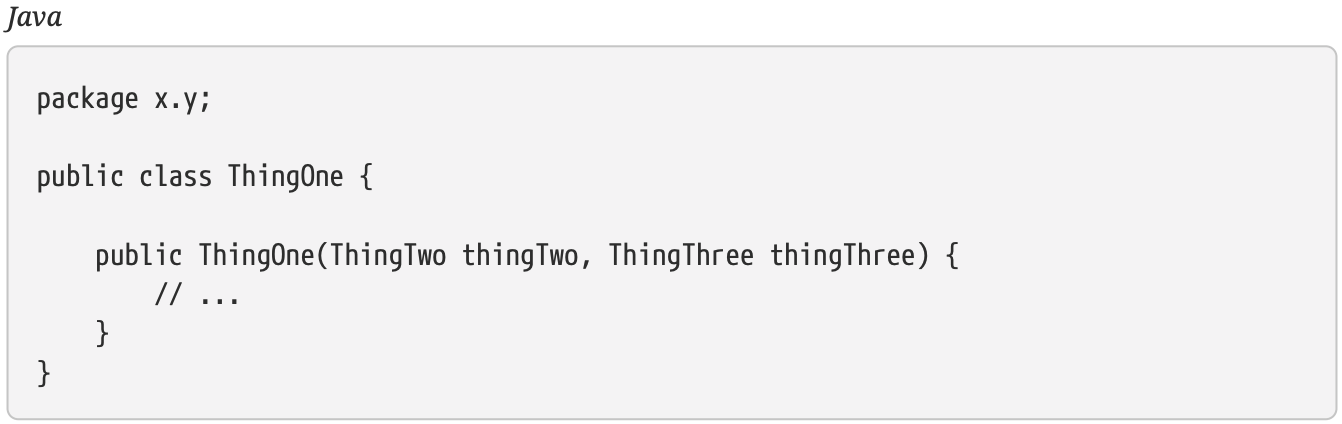
\includegraphics[width=1\linewidth]{./Figure/IMG_code_22.png}
\end{figure}
\begin{figure}[ht]
    \centering
    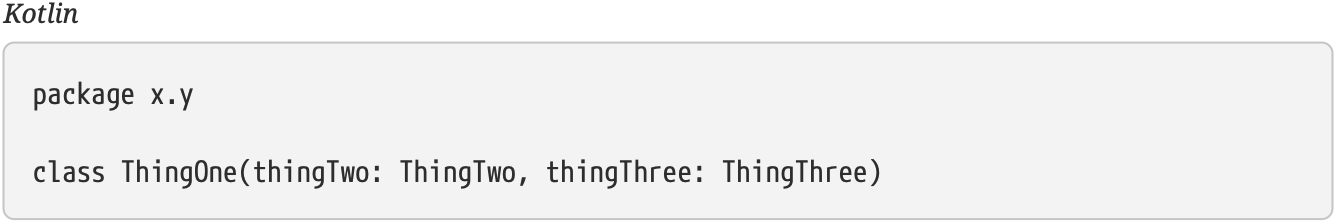
\includegraphics[width=1\linewidth]{./Figure/IMG_code_23.png}
\end{figure}

假设ThingTwo和ThingThree类没有通过继承关联,则不存在潜在的歧义。 因此,以下配置可以正常工作,并且无需在<constructor-arg />元素中显式指定构造函数参数索引或类型。

\begin{figure}[ht]
    \centering
    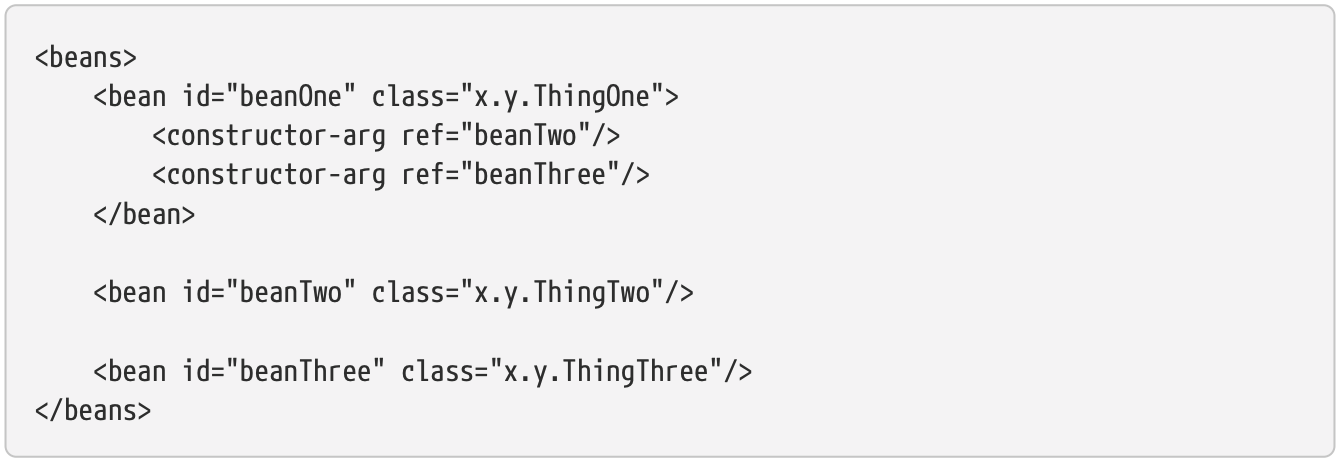
\includegraphics[width=1\linewidth]{./Figure/IMG_code_24.png}
\end{figure}

当引用另一个bean时,类型是已知的,并且可以发生匹配(与前面的示例一样)。 当使用简单类型(例如<value> true </ value>)时,Spring无法确定值的类型,因此在没有帮助的情况下无法按类型进行匹配。 考虑以下类:
\begin{figure}[ht]
    \centering
    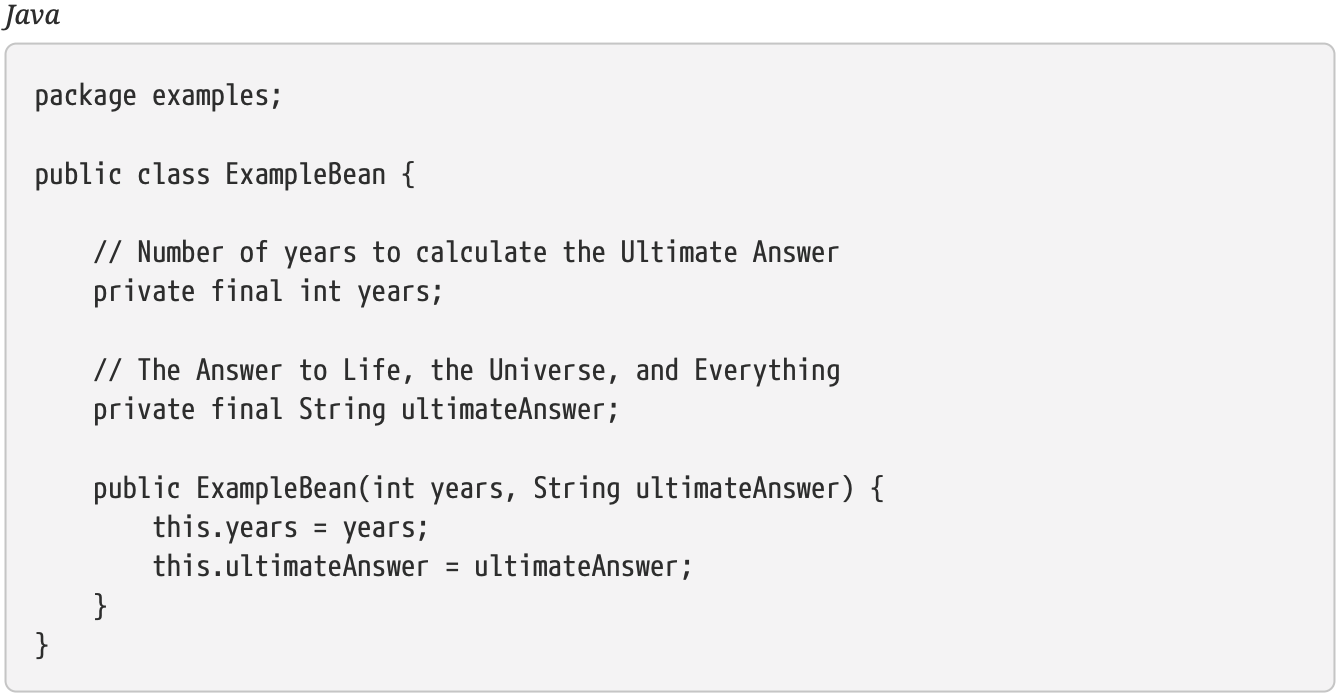
\includegraphics[width=1\linewidth]{./Figure/IMG_code_25.png}
\end{figure}

\begin{figure}[ht]
    \centering
    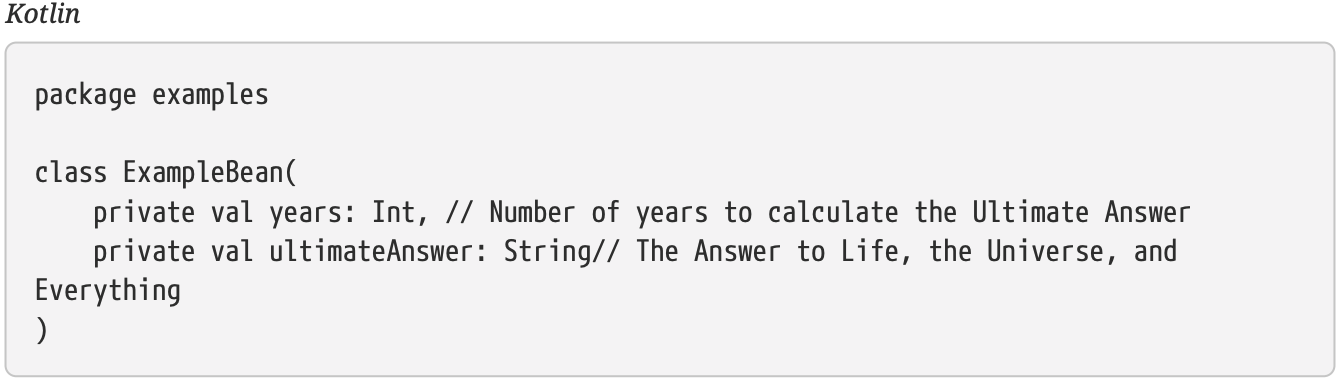
\includegraphics[width=1\linewidth]{./Figure/IMG_code_26.png}
\end{figure}


\noindent \small{\textbf{构造函数参数类型匹配}}

在上述情况下,如果通过使用type属性显式指定构造函数参数的类型,则容器可以使用简单类型的类型匹配,如以下示例所示:

\begin{figure}[ht]
    \centering
    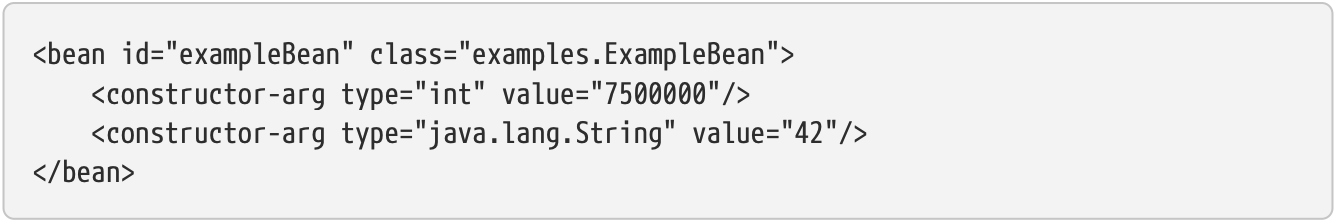
\includegraphics[width=1\linewidth]{./Figure/IMG_code_27.png}
\end{figure}

\newpage

\noindent \small{\textbf{构造函数参数索引}}

可以使用index属性来显式指定构造函数参数的索引,如以下示例所示:

\begin{figure}[ht]
    \centering
    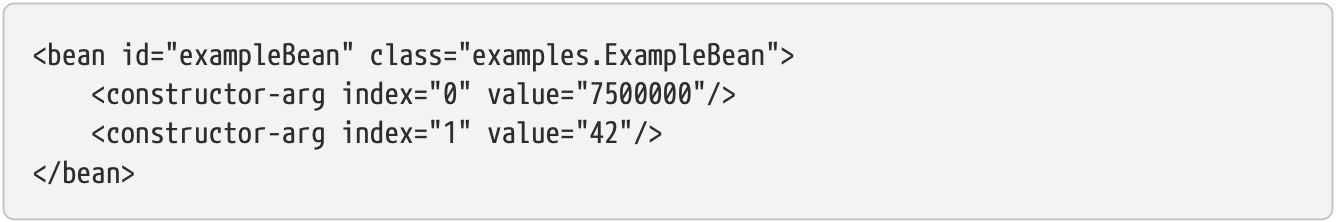
\includegraphics[width=1\linewidth]{./Figure/IMG_code_28.png}
\end{figure}

除了解决多个简单值的歧义性之外,当构造函数具有两个相同类型的参数时,指定索引还可以解决歧义。

\textbf{索引从0开始}。
\newpage
\noindent \small{\textbf{构造函数参数名称}}

还可以使用构造函数参数名称来消除歧义,如以下示例所示:

\begin{figure}[ht]
    \centering
    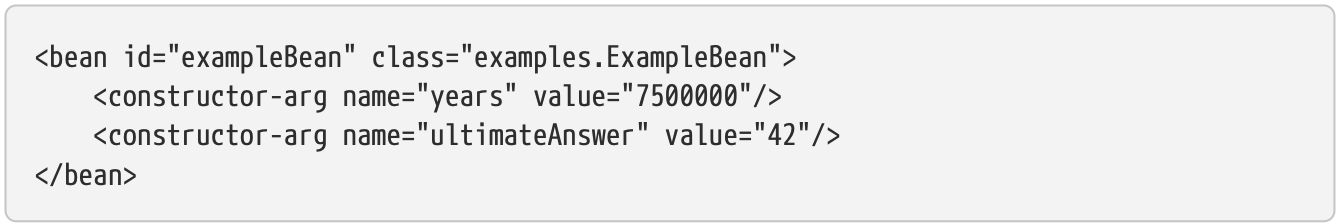
\includegraphics[width=1\linewidth]{./Figure/IMG_code_29.png}
\end{figure}

请记住,要立即使用该功能,必须在启用调试标志的情况下编译代码,以便Spring可以从构造函数中查找参数名称。 如果您不能或不想使用debug标志编译代码,则可以使用@ConstructorProperties JDK注释显式命名构造函数参数。 类必须如下所示:

\begin{figure}[ht]
    \centering
    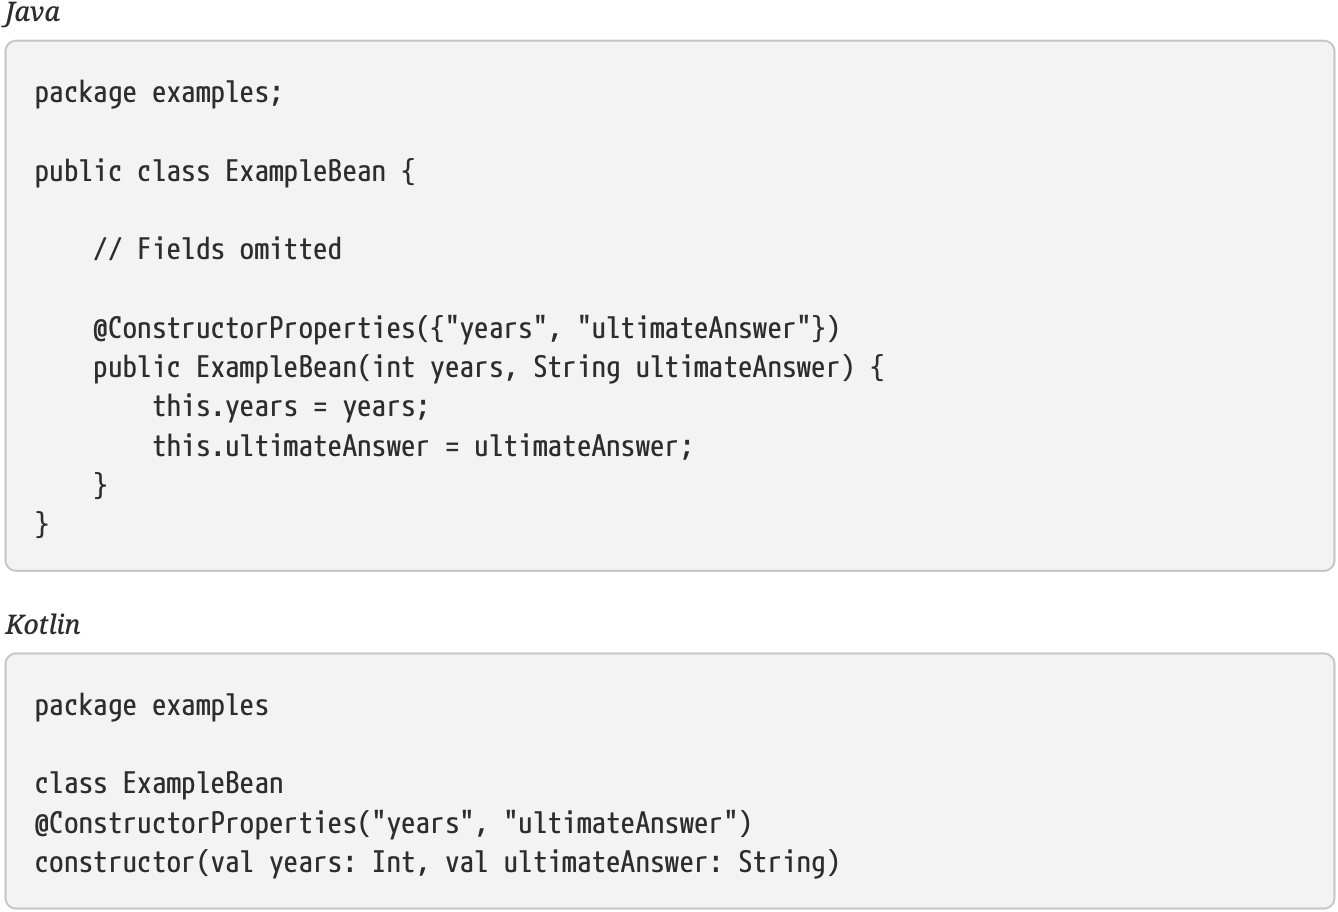
\includegraphics[width=1\linewidth]{./Figure/IMG_code_30.png}
\end{figure}

\newpage
\subsubsection{基于Setter的依赖注入}
通过调用无参数构造函数或无参数静态工厂方法以实例化的bean之后,容器通过在bean上调用setter方法来完成基于setter的DI。

下面的示例显示只能通过使用纯setter注入来进行依赖项注入的类。 此类是常规的Java。 它是一个POJO,不依赖于特定于容器的接口,基类或注解。

\begin{figure}[ht]
    \centering
    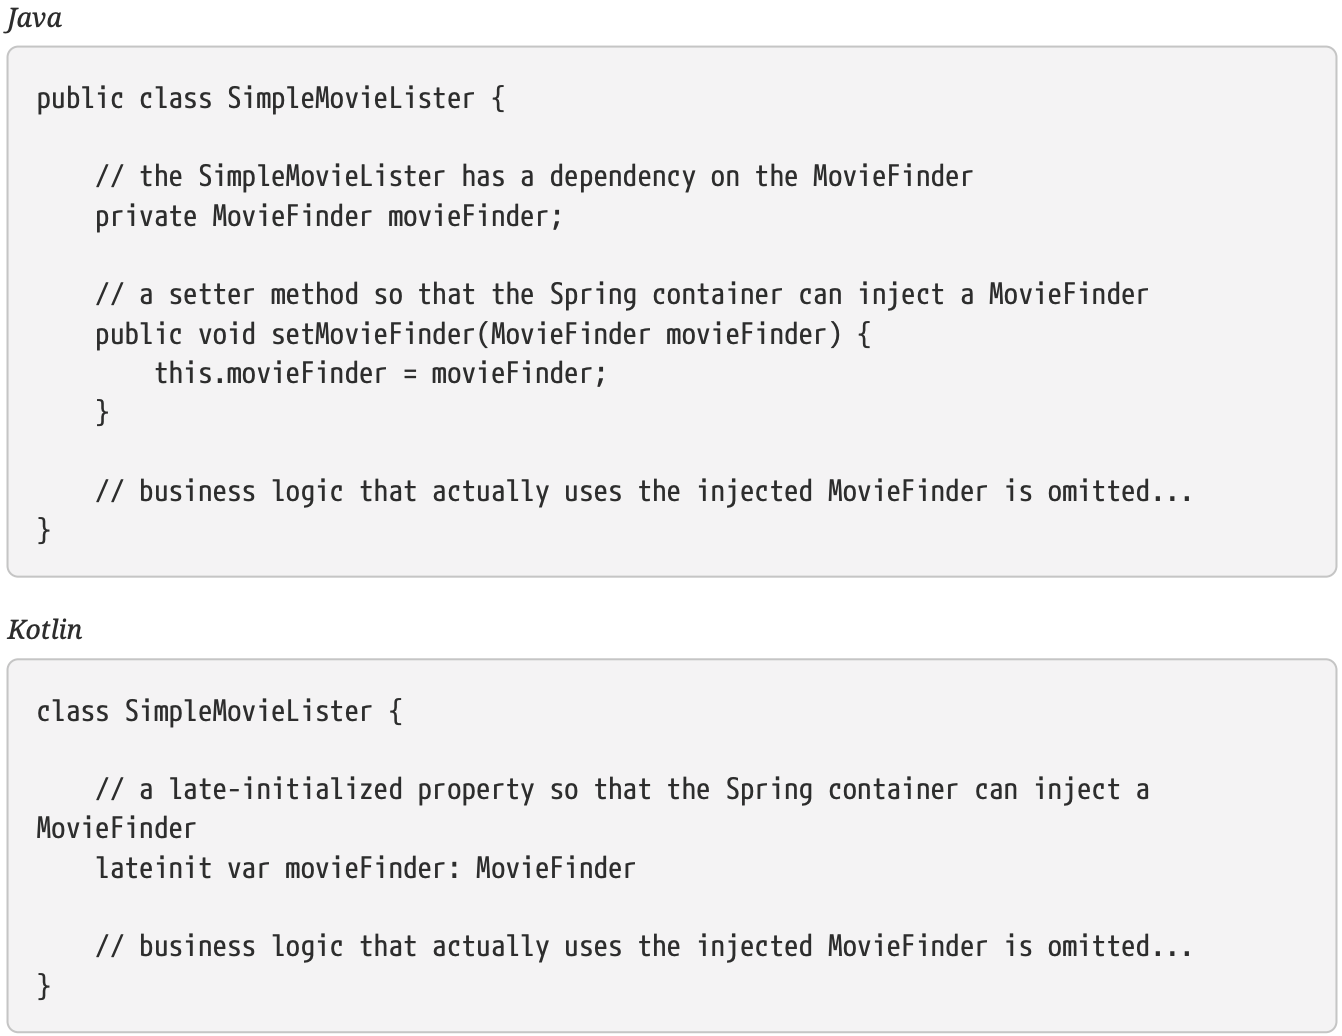
\includegraphics[width=1\linewidth]{./Figure/IMG_code_31.png}
\end{figure}

ApplicationContext为它管理的bean提供基于构造函数和基于setter的DI。
在通过构造函数方法注入了一些依赖项之后,它还支持基于setter的DI。
您可以以BeanDefinition的形式配置依赖项,与PropertyEditor实例一起使用,
将属性从一种格式转换为另一种格式。
但是,大多数Spring用户并不是直接使用这些类(即通过编程方式),而
是使用XML bean定义、带注解的组件(即使用@Component、@Controller等带注解的类),
或者基于java的@Configuration类中的@Bean方法。然后,这些源在内部转换为BeanD
efinition的实例,并用于加载整个Spring IoC容器实例。


\begin{center}
    \textbf{基于构造函数或基于setter的DI?}
\end{center}

\textit{由于可以混合使用基于构造函数的DI和基于设置setter的DI,因此,将构造函数用于强制性依赖项,将setter方法或配置方法用于可选性依赖项是一个很好的经验法则。 请注意,可以在setter方法上使用@Required批注,以使该属性成为必需的依赖项。 但是,最好使用带有参数的程序验证的构造函数注入。}

\textit{Spring团队通常提倡构造函数注入,因为它可以让您将应用程序组件实现为不可变对象,并确保所需的依赖项不为null。 此外,构造函数注入的组件始终以完全初始化的状态返回到客户端(调用)代码。 附带说明一下,大量的构造函数自变量是一种不好的代码味道,这表明该类可能承担了太多的职责,应将其重构以更好地解决关注点分离问题。}

\textit{Setter注入主要应仅用于可以在类中分配合理的默认值的可选依赖项。 否则,必须在代码使用依赖项的任何地方执行非空检查。 setter注入的一个好处是,setter方法使该类的对象在以后可以重新配置或重新注入。 因此,通过JMX MBean进行管理是使用setter注入的一个不错的用例。}

\textit{使用最适合特定Class的DI风格。 例如,如果第三方类未公开任何setter方法,则构造函数注入可能是DI的唯一可用形式。}

\subsubsection{依赖性解析过程}
容器按照如下方式执行bean依赖项解析:

\begin{itemize}
    \item 使用描述所有bean的配置元数据创建和初始化ApplicationContext。 可以通过XML,Java代码或注解来指定配置元数据。
    \item 对于每个bean,它的依赖关系以属性、构造函数参数或静态工厂方法的参数的形式表示(如果您使用静态工厂方法而不是普通构造函数)。当实际创建bean时,这些依赖项被提供给bean。
    \item 每个属性或构造函数参数都是要设置的值的实际定义,或对容器中另一个bean的引用。
    \item 作为值的每个属性或构造函数参数都将从其指定的格式转换为该属性或构造函数参数的实际类型。默认情况下,Spring可以将字符串格式提供的值转换为所有内置类型,比如int、long、string、boolean等等。
\end{itemize}

Spring容器在创建容器时验证每个bean的配置。
但是,在实际创建bean之前,不会设置bean属性本身。
单例作用域和设置为预实例化(默认)的bean会在容器被创建时是同步创建。
作用域在Bean作用域中定义。
其他类型的bean仅在请求时创建。
创建一个bean可能会导致创建多个bean
,因为需要创建bean的依赖项及其依赖项的依赖项(等等)。
请注意,这些依赖项之间的解析不匹配可能会在之后出现——即在受影响bean的第一次创建时出现。

\begin{center}
    \textbf{循环依赖}
\end{center}

\textit{如果大部分使用构造函数注入,则可能会创建无法解决的循环依赖方案。}

\textit{例如:A类通过构造函数注入需要B类的实例,而B类通过构造函数注入需要A类的实例。 如果您为类A和B配置为相互注入的bean,则Spring IoC容器会在运行时检测到此循环引用,并抛出BeanCurrentlyInCreationException。}

\textit{一种可能的解决方案是编辑某些类的源代码,这些类将由setter而不是构造函数来配置。 或者,避免构造函数注入,而仅使用setter注入。 换句话说,尽管不建议这样做,但是您可以使用setter注入配置循环依赖关系。}

\textit{与典型情况(没有循环依赖关系)不同,bean A和bean B之间的循环依赖关系迫使其中一个Bean在完全完全初始化之前被注入另一个Bean(经典的“鸡与蛋”场景)。}

您通常可以相信Spring会做正确的事情。
它在容器加载时检测配置问题,比如对不存在的bean和循环依赖项的引用。
当bean实际创建时,Spring会尽可能晚地设置属性并解析依赖项。
这意味着,如果在创建对象或其某个依赖项时出现问题,已经正确加载的Spring容器可以生成异常——例如,
bean会由于缺少或无效的属性而抛出异常。这可能会延迟一
些配置问题的可见性,这就是为什么ApplicationContext实
现默认情况下会预先实例化单例bean。在实际需要这些bean之前
创建这些bean需要花费一些前期时间和内存,但是在创建Appli
cationContext时就可以发现配置问题。
这个默认行为可以被覆盖,使单例bean的初始化延迟。

如果不存在循环依赖项,那么当一个或多个协作bean被注入到依赖bean中时,
每个协作bean在被注入到依赖bean之前都会被完全配置。这
意味着,如果bean A依赖于bean B, Spring IoC容器在调用bean A
的setter方法之前完全配置bean B。换句话说,当bean已经被实例化(如果它不
是一个预实例化的单例),那么它的依赖项就已经被设置,并且相关的生命周期方法也已经被调用
(例如配置的init方法或InitializingBean回调方法)。

\subsubsection{依赖注入的例子}
\newpage
\subsection{依赖和配置的细节}
如上一节所述,您可以将bean属性和构造函数参数定义为对其他托管bean(协作者)的引用,也可以定义为内联定义的值。 Spring的基于XML的配置元数据为此目的在其<property />和<constructor-arg />元素中支持子元素类型。

\subsubsection{常量(原始类型、字符串等)}

</property>元素的value属性将属性或构造函数参数指定为人类可读的字符串表示形式。Spring的转换服务用于将这些值从String转换为属性或参数的实际类型。下面的示例显示了正在设置的各种值:

\begin{figure}[ht]
    \centering
    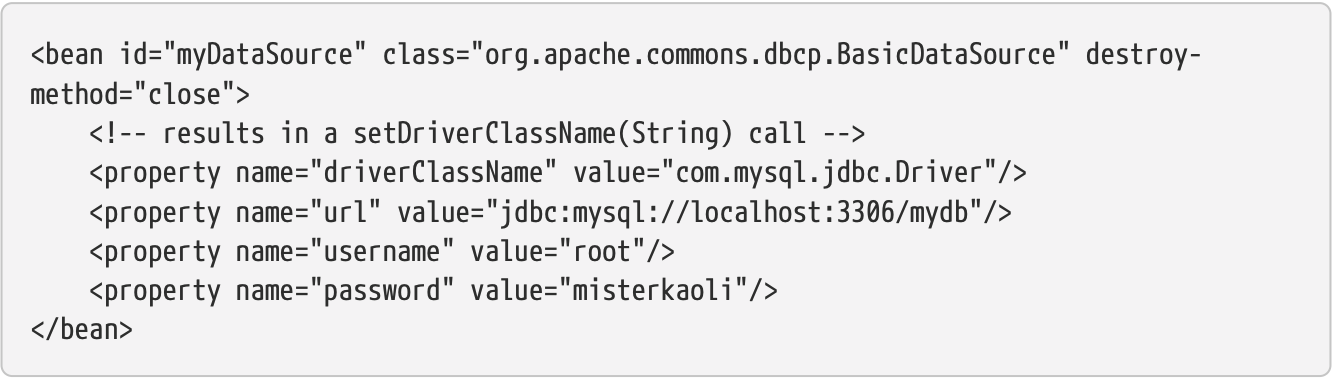
\includegraphics[width=1\linewidth]{./Figure/IMG_code_32.png}
\end{figure}

下面的例子使用p-namespace来进行更简洁的XML配置:

\begin{figure}[ht]
    \centering
    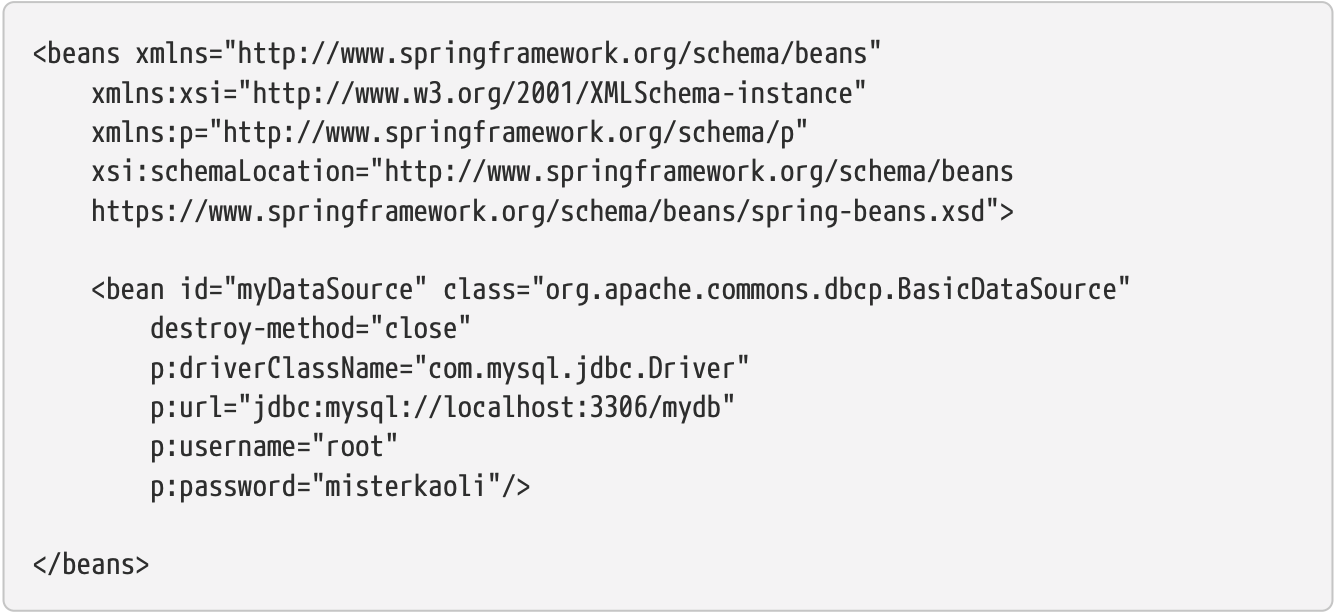
\includegraphics[width=1\linewidth]{./Figure/IMG_code_33.png}
\end{figure}

前面的XML更简洁。然而,输入错误只能在运行时被发现,除非使用支持创建bean定义时自动完成属性的IDE(如IntelliJ IDEA或用于Eclipse的Spring Tools)。强烈推荐这样的IDE帮助。

\newpage
您也可以配置一个java.util.Properties实例,如下所示:


\begin{figure}[ht]
    \centering
    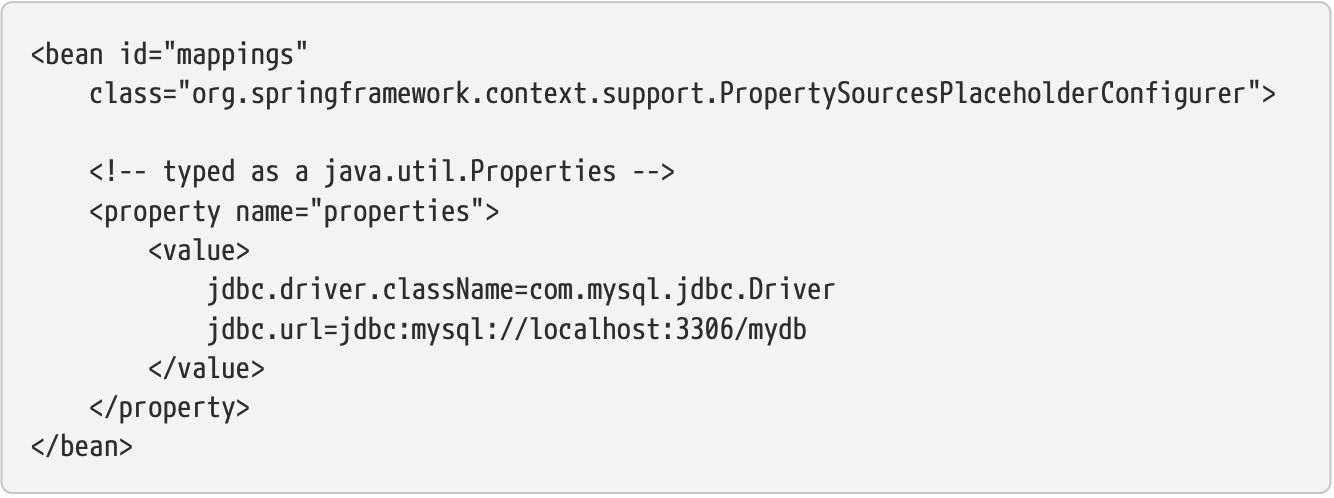
\includegraphics[width=1\linewidth]{./Figure/IMG_code_34.png}
\end{figure}

通过使用JavaBeans的PropertyEditor机制,Spring容器将<value></value>元素中的文本
转换为java.util.Properties实例。这是一个很好的快捷方式,也是
Spring团队喜欢使用嵌套<value></value>元素而不是value属性样式的少数地方之一。

\noindent \small \textbf{idref元素}

idref元素只是将容器中另一个bean的id(字符串值——而不是引用)传递给<constructor-arg>或</property>元素的一种防止错误的方法。</constructor-arg>下面的例子展示了如何使用它:

\begin{figure}[ht]
    \centering
    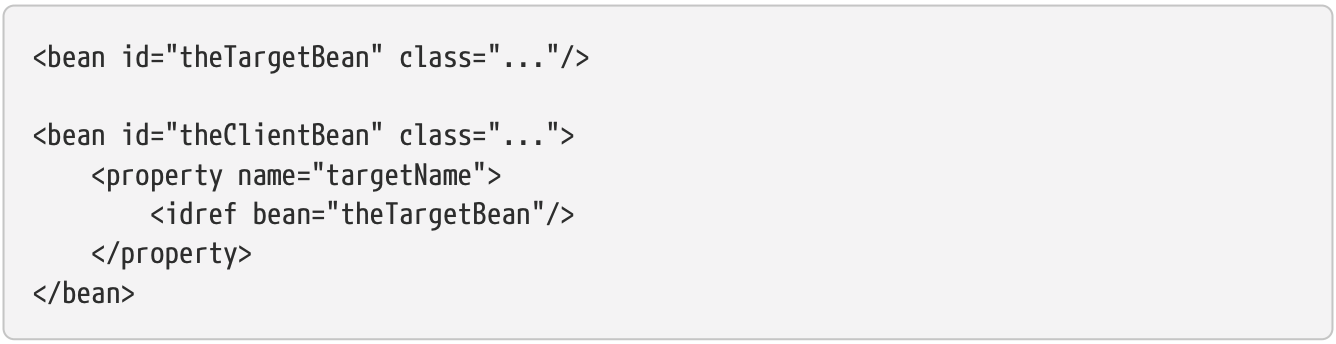
\includegraphics[width=1\linewidth]{./Figure/IMG_code_35.png}
\end{figure}

前面的bean定义片段(在运行时)与下面的片段完全相同:

\begin{figure}[ht]
    \centering
    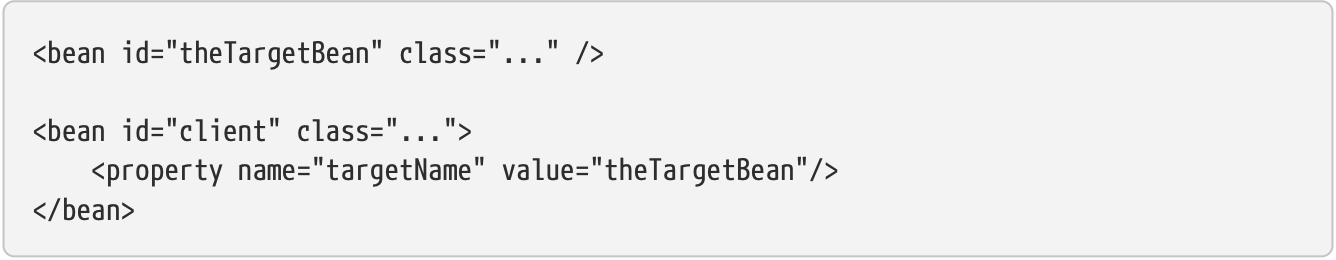
\includegraphics[width=1\linewidth]{./Figure/IMG_code_36.png}
\end{figure}

第一种形式比第二种形式更可取,因为使用idref标
记可以让容器在部署时验证所引用的已命名bean实际存在。
在第二个变体中,对传递给目标bean的targetName属性的值不执行任何验证。
只有在实际实例化目标bean时才会发现错误(很可能导致致命的结果)。如果目标bean是一个原型bean
,那么这个输入错误和由此产生的异常可能要在容器部署很久之后才会被发现。

\textbf{在4.0 Bean XSD中不再支持idref元素上的local属性,因为它不再提供常规Bean引用上的值。 升级到4.0模式时,将现有的idref本地引用更改为idref bean。}


<idref></idref>元素的一个常见地方(至少在Spring 2.0之前的版本中)
是在ProxyFactoryBean bean定义中的AOP拦截器配置中。在指定拦截器名称时
使用<idref></idref>元素可以防止拼错写错误。

\subsubsection{对其他bean(合作者)的引用}
ref元素是<constructor-arg>或</property>定义元素中的最后一个元素。
您将一个bean的指定属性的值设置为对容器管
理的另一个bean(合作者)的引用。被引用的bean是要设置其属性的bean的依赖
项,在设置属性之前,根据需要对其进行初始化。(如果合作者是一个单例bean,
它可能已经被容器初始化了。)所有引用最终都是对另一个对象的引用。范围和验
证取决于您是通过bean还是父属性指定其他对象的ID或名称。

通过<ref></ref>标记bean属性来指定目标bean是最通用的形式,
允许在同一容器或父容器中创建对任何bean的引用,
而不管它是否在同一XML文件中。
bean属性的值可以与目标bean的id属性相同,
也可以与目标bean的name属性中的某个值相同。
下面的例子展示了如何使用ref元素:

\begin{figure}[ht]
    \centering
    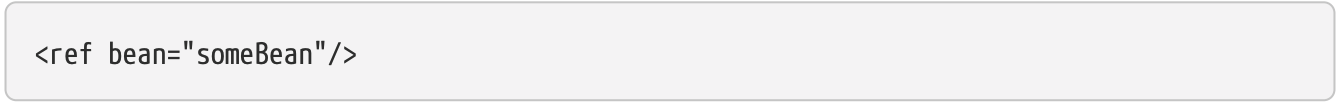
\includegraphics[width=1\linewidth]{./Figure/IMG_code_37.png}
\end{figure}

通过parent属性指定目标bean将创建对当前容器父容器中的bean的引用。
parent属性的值可以与目标bean的id属性或目标bean的name属性中的一个值相同。
目标bean必须位于当前bean的父容器中。
当您有一个容器层次结构,并且您想用与父容器中的bean同名的代理将现有它包装时,
您应该主要使用这个bean引用变体。下面的两个清单显示了如何使用parent属性:

\begin{figure}[ht]
    \centering
    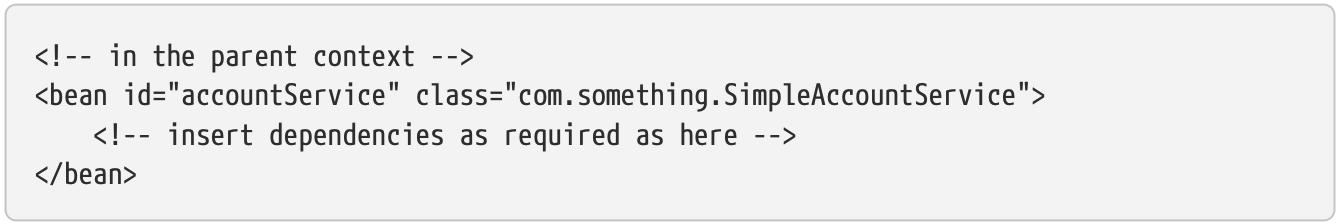
\includegraphics[width=1\linewidth]{./Figure/IMG_code_38.png}
\end{figure}

\newpage
\begin{figure}[ht]
    \centering
    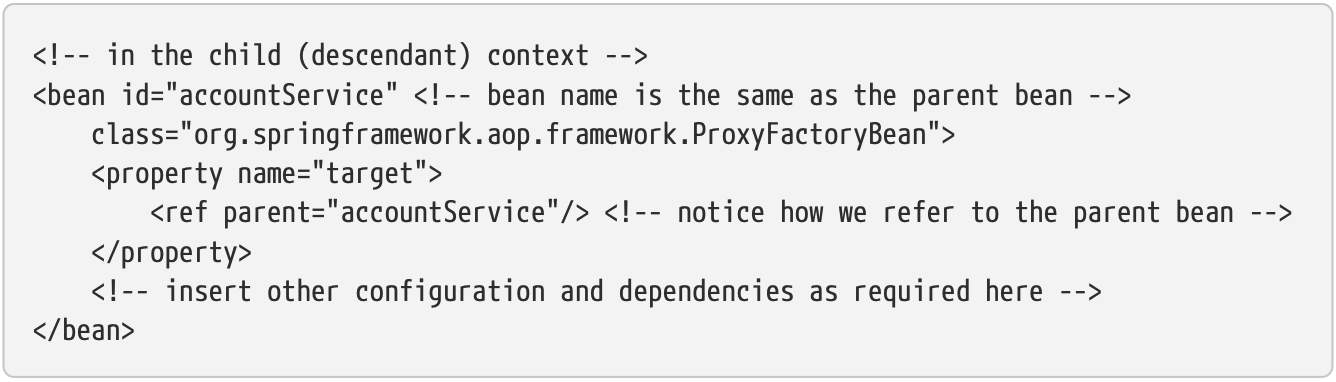
\includegraphics[width=1\linewidth]{./Figure/IMG_code_39.png}
\end{figure}


\textbf{ref元素的local属性在4.0 Bean XSD中不再受支持,因为它不再提供常规Bean引用上的值。 升级到4.0模式时,将现有的ref本地引用更改为ref bean。}

\subsubsection{内部Bean}
<property />或<constructor-arg />元素内的<bean />元素定义了一个内部bean,如以下示例所示:

\begin{figure}[ht]
    \centering
    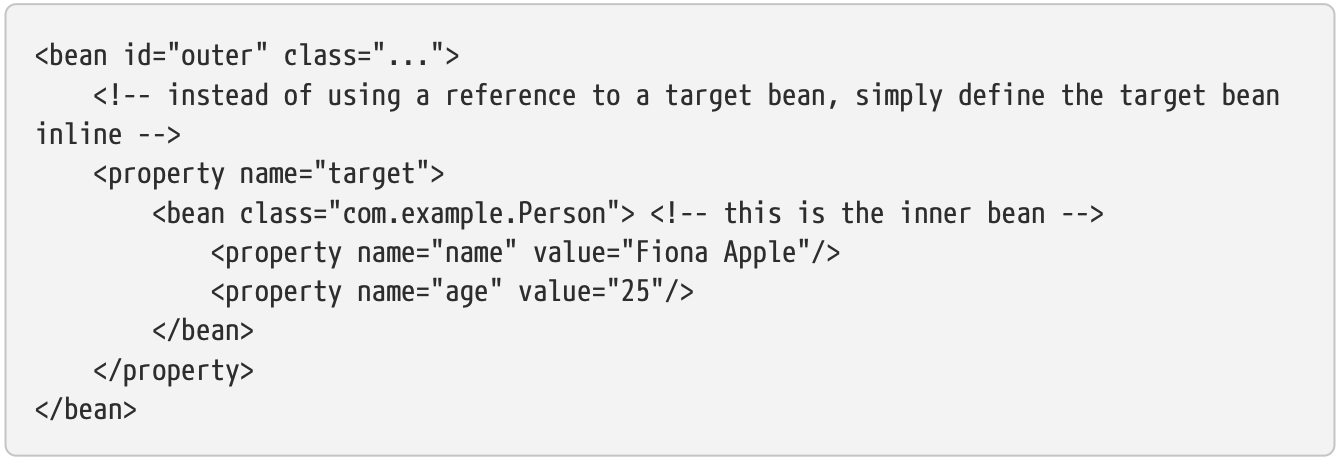
\includegraphics[width=1\linewidth]{./Figure/IMG_code_40.png}
\end{figure}

内部bean定义不需要定义的ID或名称。
如果指定,则容器不使用该值作为标识符。
容器在创建时也将忽略作用域标志,
因为内部Bean始终是匿名的,并且始终与外部Bean一起创建。
不可能独立访问内部bean或将它们注入到其他协作的bean中。

作为一个极端的例子,可以从自定义范围接收破坏回调,
例如,针对单例bean中包含的请求范围内的bean。 
内部bean实例的创建与其包含的bean绑定在一起,
但是销毁回调使它可以参与请求范围的生命周期。 
这不是常见的情况。 内部bean通常只共享其包含bean的作用域。

\newpage
\subsubsection{集合}
<list />,<set />,<map />和<props />元素分别对应Java集合类型的
List,Set,Map和Properties。 以下示例显示了如何使用它们:

\begin{figure}[ht]
    \centering
    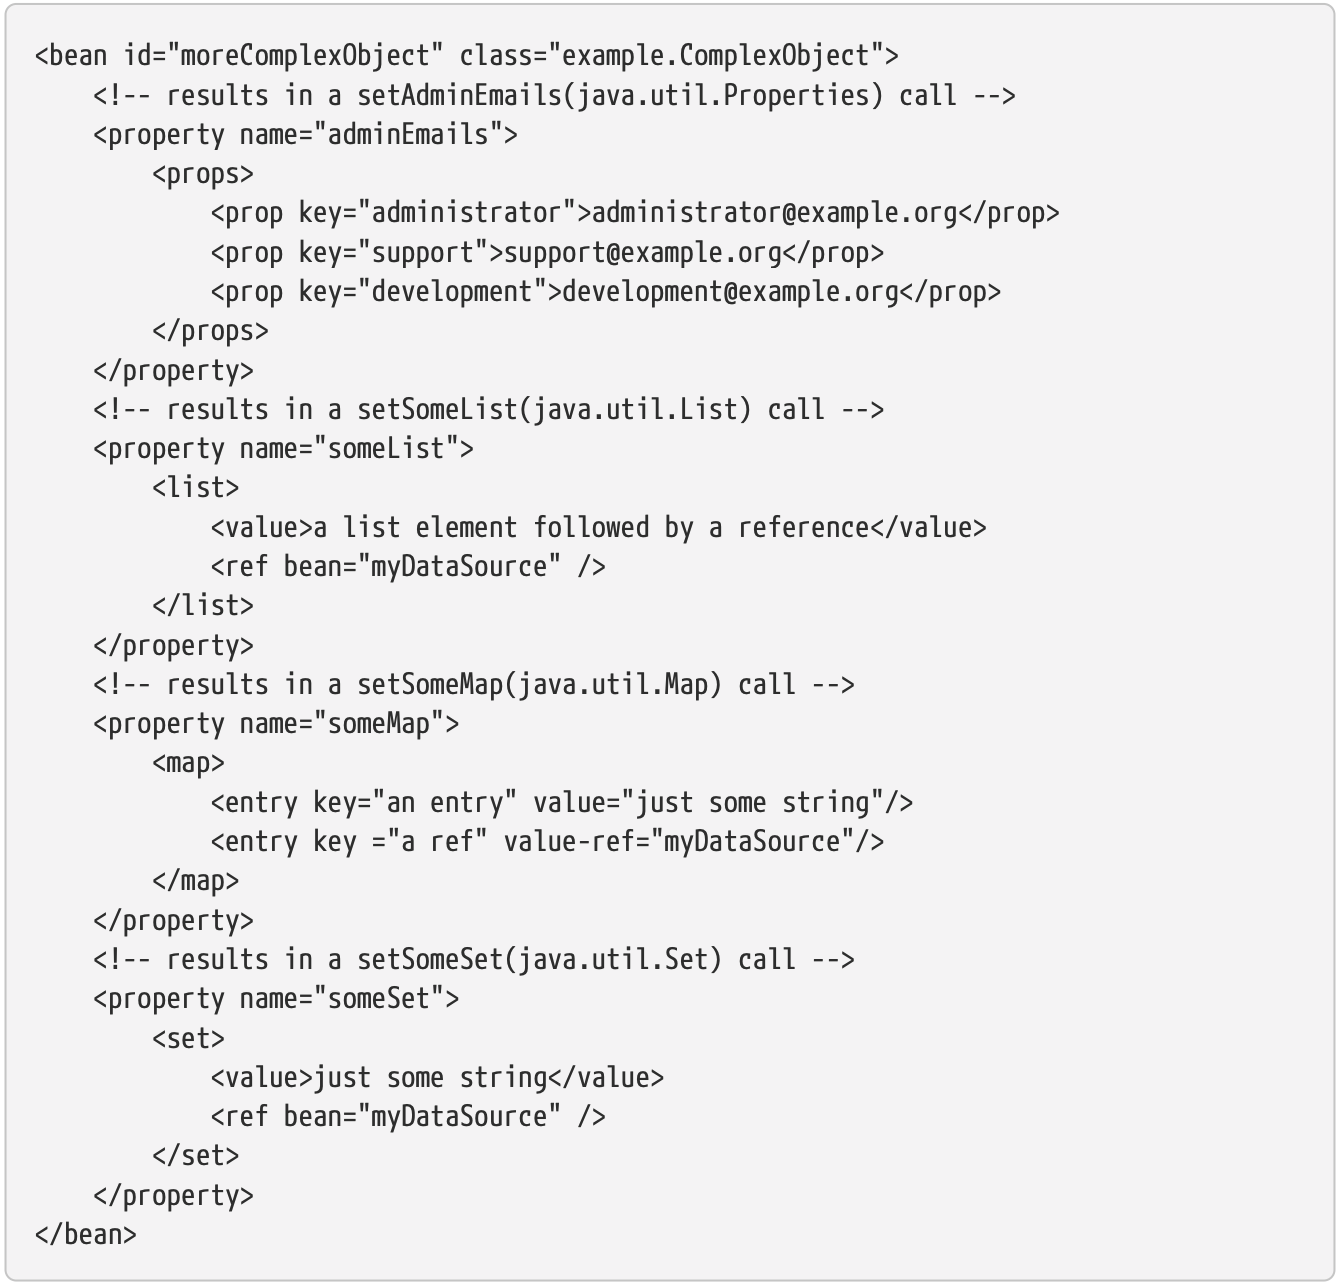
\includegraphics[width=1\linewidth]{./Figure/IMG_code_41.png}
\end{figure}

Map 的 键和值、Set的值可以是一下几种之一:

\begin{figure}[ht]
    \centering
    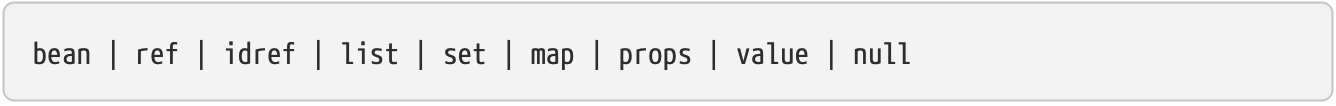
\includegraphics[width=1\linewidth]{./Figure/IMG_code_42.png}
\end{figure}

\noindent \small \textbf{集合合并}

Spring容器还支持合并集合。应用程序开发人员可以定义父<list/>、<map/>、<set/>或<props/>元素,并让子<list/>、<map/>、<set/>或<props/>元素继承和重写父集合中的值。也就是说,子集合的值是合并父集合和子集合的元素的结果,子集合的元素将覆盖父集合中指定的值。

这部分关于合并的内容会涉及到父子bean机制。
不熟悉父bean和子bean定义的读者可能希望在继续之前阅读相关部分。

以下示例演示集合合并:

\begin{figure}[ht]
    \centering
    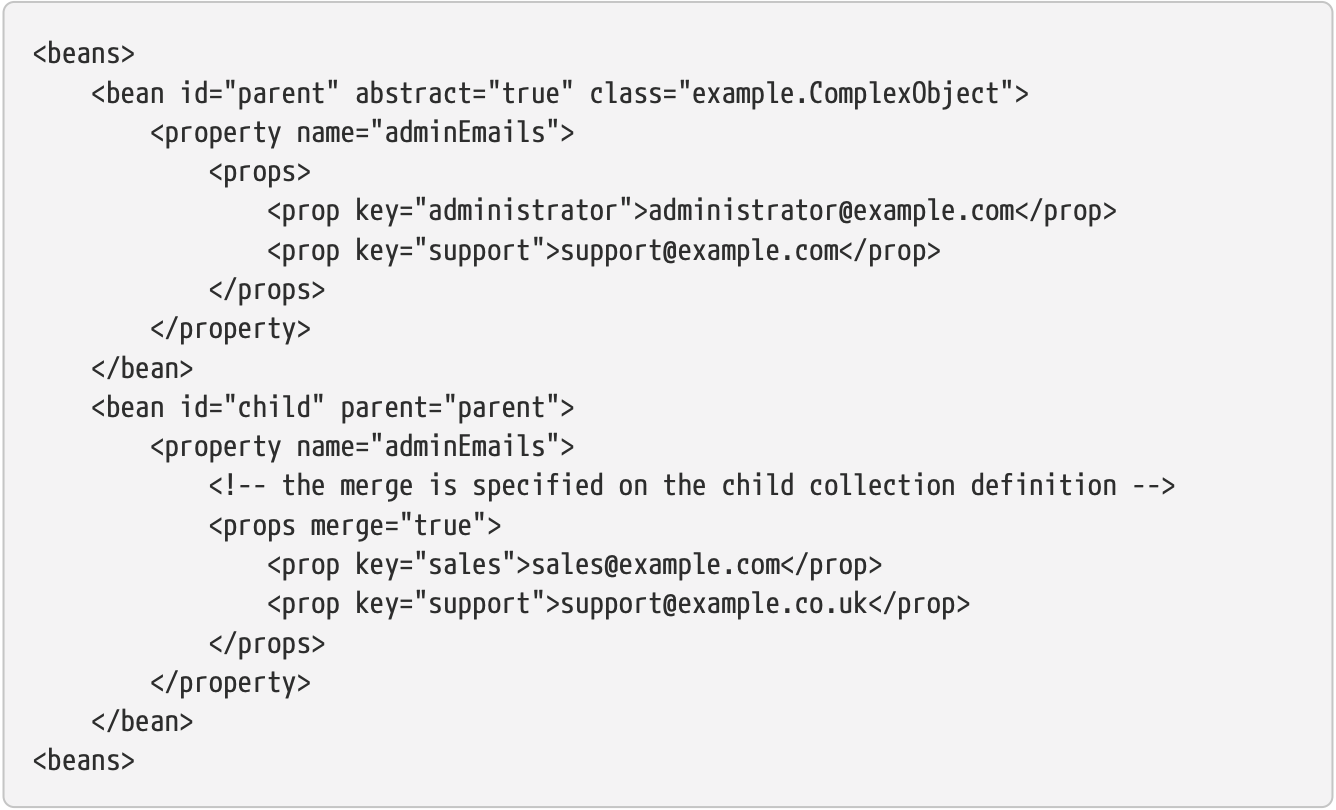
\includegraphics[width=1\linewidth]{./Figure/IMG_code_43.png}
\end{figure}

注意,在子bean定义的adminEmails属性的<props/>元素上使用了merge=true属性。当容器解析并实例化子bean时,生成的实例具有一个adminEmails属性集合,该集合包含将子级的adminEmails集合与父级的adminEmails集合合并的结果。下面的列表显示了结果:

\begin{figure}[ht]
    \centering
    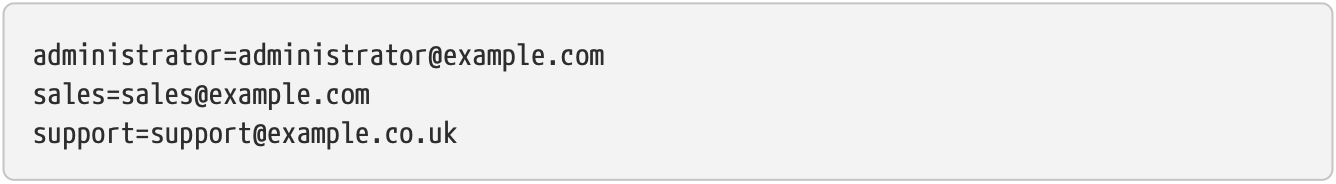
\includegraphics[width=1\linewidth]{./Figure/IMG_code_44.png}
\end{figure}


子Bean拥有所有父Bean在<props/> 中定义的元素,同时子Bean的<props/>中的元素会覆盖父Bean的值。

此合并行为类似地适用于<list/>、<map/>和<set/>集合类型。
在<list/>元素的特定情况下,与列表集合类型相关联的语义会被(即,值的有序集合的概念)得到维护。
父列表的值在所有子列表的值之前。
对于Map、Set和Properties集合类型,不存在排序。
因此,对于容器内部使用的关联Map、Set和Properties实现类型下面的集合类型,没有有效的排序语义。

\noindent \small \textbf{集合合并的局限性}

不能合并不同的集合类型(如Map和List),这样会引发相应的异常。
必须在子定义上指定merge属性,在父集合定义上指定merge属性是无效的,不会导致所需的合并。

\noindent \small  \textbf{强类型集合}

随着Java5中泛型类型的引入,您可以使用强类型集合。
也就是说,可以声明一个集合类型,使得它只能包含(例如)字符串元素。
如果使用Spring依赖关系将强类型集合注入bean,
则可以利用Spring的类型转换,
以便在将强类型集合实例的元素添加到集合之前将其转换为适当的类型。
下面的Java类和bean定义演示了如何执行此操作:

\begin{figure}[ht]
    \centering
    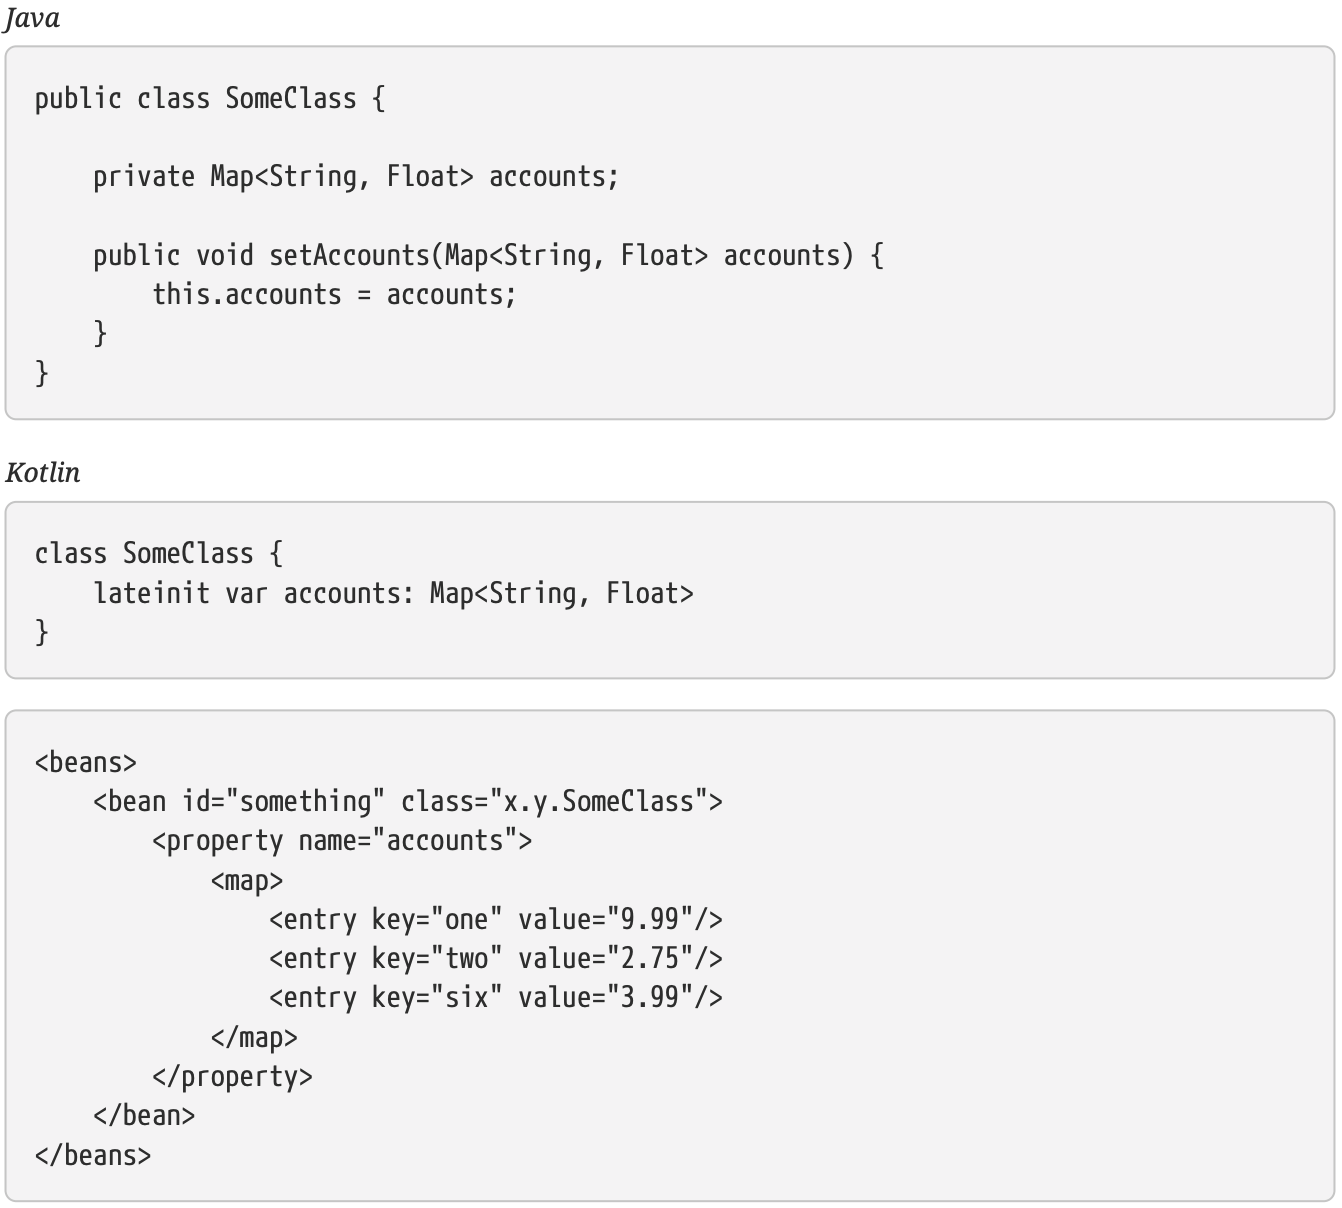
\includegraphics[width=1\linewidth]{./Figure/IMG_code_45.png}
\end{figure}

当something bean的accounts属性准备好注入时,
关于强类型Map<String,Float>的元素类型的泛型信息可以通过反射获得。
因此,Spring的类型转换将各种值元素识别为Float类型,
字符串值(9.99、2.75和3.99)被转换为实际的Float类型。

\newpage
\subsubsection{Null和空字符串值}
Spring将属性等的空参数视为空字符串。以下基于XML的配置元数据片段将email属性设置为空字符串值(“”)。

\begin{figure}[ht]
    \centering
    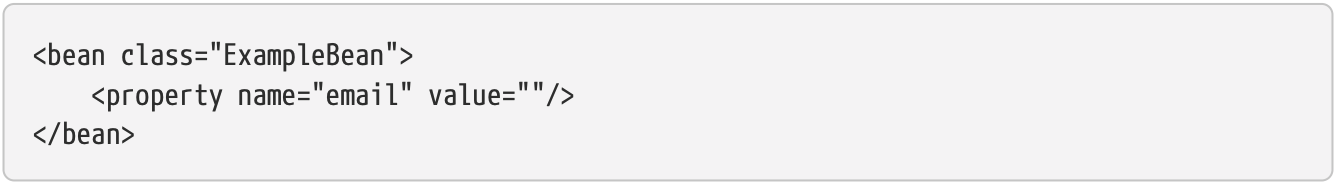
\includegraphics[width=1\linewidth]{./Figure/IMG_code_46.png}
\end{figure}

前面的示例等效于以下Java代码:

\begin{figure}[ht]
    \centering
    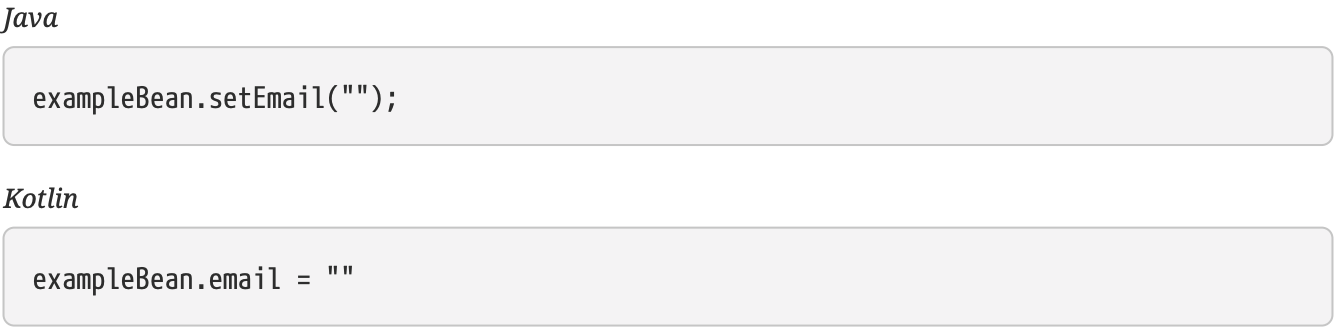
\includegraphics[width=1\linewidth]{./Figure/IMG_code_47.png}
\end{figure}

<null />元素代表空值。 如下代码所示:

\begin{figure}[ht]
    \centering
    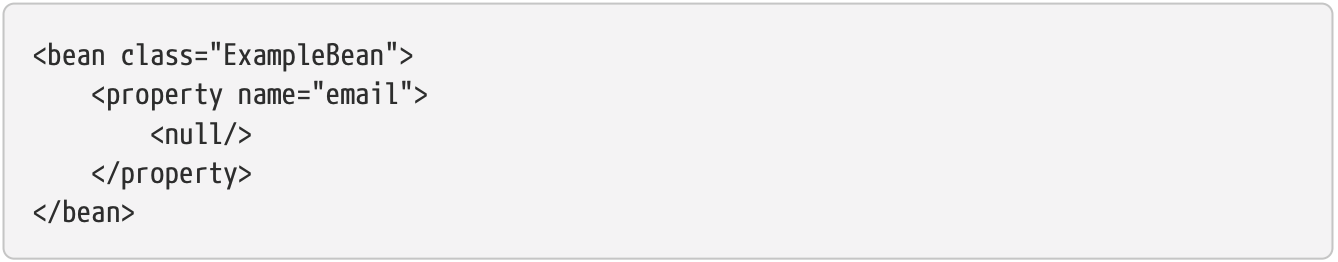
\includegraphics[width=1\linewidth]{./Figure/IMG_code_48.png}
\end{figure}

\newpage
前面的示例等效于以下Java代码:

\begin{figure}[ht]
    \centering
    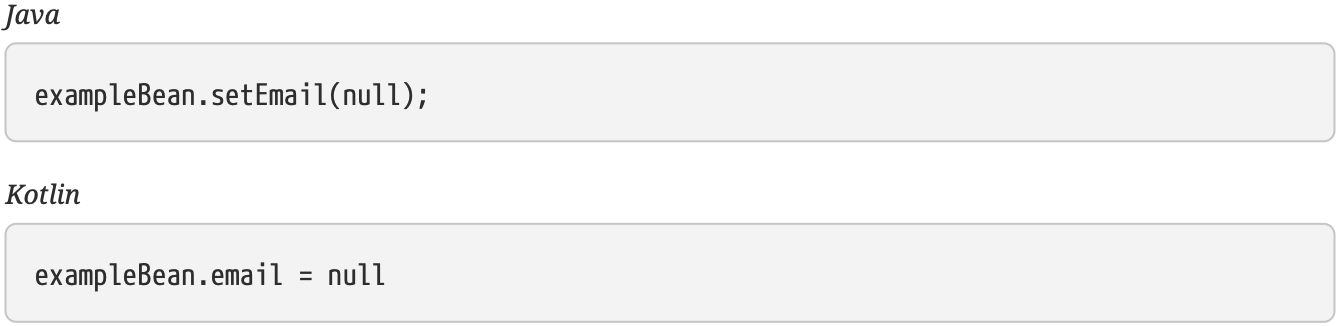
\includegraphics[width=1\linewidth]{./Figure/IMG_code_49.png}
\end{figure}

\subsubsection{p-namespace的XML快捷配置}
使用p-namespace,就可以使用<bean/>标签的元素来描述
bena的属性值(而不是嵌套的<property />元素)。

Spring支持带有名称空间的可扩展配置格式,这些名称空间基于XML Schema定义。 本章讨论的bean配置格式是在XML Schema文档中定义的。 但是,p命名空间未在XSD文件中定义,仅存在于Spring的核心中。

下面的示例显示了两个XML代码段(第一个使用标准XML格式,第二个使用p-命名空间),它们可以解析为相同的结果:

\begin{figure}[ht]
    \centering
    \includegraphics[width=1\linewidth]{./Figure/IMG_code_50.png}
\end{figure}

该示例显示了使用p命名空间
配置了bean 定义的email属性。
如前所述,p命名
空间没有架构定义,因此可以将属性名称写在“p” 之后。
\newpage
下一个示例包括另外两个bean定义,它们都引用了另一个bean:

\begin{figure}[ht]
    \centering
    \includegraphics[width=1\linewidth]{./Figure/IMG_code_51.png}
\end{figure}

此示例不仅包括使用p-namespace的属性值,而且还使用特殊格式来声明属性引用。 
第一个bean定义使用<property name =“ spouse” ref =“ jane” />创建从bea
n john到bean jane的引用,而第二个bean定义使用p:spouse-ref =“ jane”作为
属性来配置,其实作用想用。 在这种情况下,spouse是属性名称,而-ref部分指示这不是
一个直接值,而是对另一个bean的引用。

\textbf{p命名空间不如标准XML格式灵活。 例如,用于声明属性引用的格式与以Ref结尾的属性发生冲突,而标准XML格式则没有。 我们建议您谨慎选择方法,并将其传达给团队成员,以避免同时使用这三种方法生成XML文档。}

\subsubsection{c-namespace的XML快捷配置}

与带有p-namespace的XML快捷方式类似,spring3.1中引入的c-namespace允许内联属性来配置构造函数参数,而不是嵌套的constructorarg元素。
\newpage
下面的示例使用c:命名空间执行与基于构造函数的依赖项注入相同的操作:

\begin{figure}[ht]
    \centering
    \includegraphics[width=1\linewidth]{./Figure/IMG_code_52.png}
\end{figure}

c:namespace使用与p命名空间
相同的约定来按名称设置构造函数参数。
类似地,它需要在XML文件中声明,因为它没有在XSD模式中定义(它仅存在于Spring内核中)。


对于构造函数参数名称不可用的罕见情况(通常是在编译字节码时没有调试信息),可以使用回退到参数索引,如下所示:

\begin{figure}[ht]
    \centering
    \includegraphics[width=1\linewidth]{./Figure/IMG_code_53.png}
\end{figure}

\textbf{由于XML语法的原因,索引符号要求前导\_的存在,因为XML属性名称不能以数字开头(即使某些IDE允许)。 相应的索引符号也可用于<constructor-arg>元素,但并不常用,因为声明的普通顺序通常就足够了。}

实际上,构造函数解析机制在匹配参数方面非常有效,因此除非您真的需要,否则我们建议在整个配置中使用名称表示法。

\subsubsection{复合属性名}
设置bean属性时,可以使用复合或嵌套属性名,只要路径中除最终属性名以外的所有部分都不为null。考虑以下bean定义:

\begin{figure}[ht]
    \centering
    \includegraphics[width=1\linewidth]{./Figure/IMG_code_54.png}
\end{figure}

something bean有一个fred属性,
fred有一个bob属性,
bob有一个sammy属性,最后sammy属性的值被设置为123。
在构造bean之后,something的fred属性和fred的bob属性不能为null,否则将抛出NullPointerException。

\subsection{使用 depends-on}
如果一个bean是另一个bean的依赖项,这通常意味着一个bean被设置为另一个bean的属性。
通常,您可以通过基于XML的配置元数据中的<ref/>元素来实现这一点。然而,有时bean之间的依赖关系不那么直接。例如,当需要触发类中的静态初始值设定项时,例如数据库驱动程序注册。depends-on属性可以显式地强制在初始化使用此元素的bean之前初始化一个或多个bean。以下示例使用depends-on属性表示对单个bean的依赖关系:

\begin{figure}[ht]
    \centering
    \includegraphics[width=1\linewidth]{./Figure/IMG_code_55.png}
\end{figure}

要表示对多个bean的依赖关系,请提供一个bean名称列表作为dependson属性的值(逗号、空格和分号是有效的分隔符):

\begin{figure}[ht]
    \centering
    \includegraphics[width=1\linewidth]{./Figure/56.png}
\end{figure}

\textbf{Depends-on属性既可以指定初始化时间相关性,也可以在单例bean的情况下指定相应的销毁时间相关性。 与给定bean定义依赖关系的从属bean首先被销毁,然后再销毁给定bean本身。 因此,depends-on也可以控制关闭顺序。}

\subsection{懒加载Bean}

默认情况下,ApplicationContext实现会在初始化过程中创建和配置所有单例bean。
通常,这种预实例化是可取的,因为配置或周围环境中的错误是立即发现的,而不是几小时甚至几天后才发现的。当这种行为不可取时,您可以通过将bean定义标记为懒加载来防止单例bean的预实例化。延迟初始化bean告诉IoC容器在第一次请求时创建bean实例,而不是在启动时。

在XML中,此行为由<bean/>元素上的lazy init属性控制,如下例所示:

\begin{figure}[ht]
    \centering
    \includegraphics[width=1\linewidth]{./Figure/57.png}
\end{figure}

当上述配置被ApplicationContext使用时,当ApplicationContext启动时,懒加载bean不会被立刻实例化,而非懒加载bean会被立刻实例化。

然而,当一个懒加载bean是一个非懒加载的单例bean的依赖项时,ApplicationContext会在启动时创建懒加载的bean,因为它必须满足单例bean的依赖项。懒加载的bean被注入到其他非懒加载的单例bean中。

您还可以使用<beans/>元素上的default-lazy-init属性在容器级别控制延迟初始化,如下例所示:

\begin{figure}[ht]
    \centering
    \includegraphics[width=1\linewidth]{./Figure/58.png}
\end{figure}

\subsection{自动装配依赖项}
Spring容器可以自动关联依赖bean之间的关系。
通过查找ApplicationContext内的Bean,
可以让Spring自动为bean注入依赖(其他bean)。自动装配依赖项具有以下优点:


\begin{itemize}
    \item 自动关联可以显著减少指定属性或构造函数参数的需要(在这方面,本章其他地方讨论的其他机制(如bean模板)也很有价值。)
    \item 随着对象增加,自动装配可以更新配置。
     例如,如果您需要向类中添加依赖项,则无需修改配置即可自动满足该依赖项。 
     因此,自动装配在开发过程中特别有用,并不需要在代码库变得更稳定时切换到显式接线的选择。
\end{itemize}

使用基于XML的配置元数据时(请参阅“依赖注入”),可以使用<bean />元素的aut
owire属性为bean定义指定自动装配模式。 自动装配功能具有四种模式。 您
可以为每个bean指定自动装配。 下文描述了四种自动装配模式:

\begin{itemize}
    \item \textbf{no}:(默认)无自动装配。Bean引用必须由ref元素定义。对于较大的系统,不建议更改默认设置,因为显式指定协作者可以提供更大的控制和清晰度。在某种程度上,它记录了一个系统的结构。
    \item \textbf{byName}:按属性名称自动关联。Spring寻找与需要自动连接的属性同名的bean。例如,如果bean定义按属性名称自动装配,并且它包含一个master属性(也就是说,它有一个setMaster(..)方法),Spring将查找一个名为master的bean定义并使用它来设置属性。
    \item \textbf{byType}:如果容器中正好存在一个属性类型的bean,则允许自动装配属性。如果存在多个异常,将抛出一个致命异常,这表示您可能不会对该bean使用byType自动装配。如果没有匹配的bean,则不会发生任何事情(属性不会被设置)。
    \item \textbf{constructor}:类似于byType,但适用于构造函数参数。如果容器中没有一个符合构造函数参数类型的bean,则会引发致命错误。
\end{itemize}

byType和constructor自动装配模式可以装配数组和范型集合。
在这种情况下,将提供容器中与预期类型匹配的所有可以自动装配的候选对象以满足依赖关系。
如果所需的键类型为String,则可以自动装配强类型的Map。
自动装配的Map的值由与预期类型匹配的所有bean实例组成,Map的键包含相应的bean名称。

\subsubsection{自动装配的局限性和缺点}
最好在项目中的所有地方使用自动装配,否则会让其他开发人员感到困惑。

考虑自动装配的限制和缺点:
\begin{itemize}
    \item 属性和构造函数参数设置中的显式依赖项始终会覆盖自动装配的结果。
    不能自动装配原始类型、字符串和类(以及它们构成的数组)等简单属性,此限制是设计使然。
    \item 自动装配不如显式装配精确。 尽管如前所述,Spring还是谨慎地避免在可能导致意外结果的模糊情况下进行猜测,对象之间的依赖关系不会那么的显而易见。
    \item 从Spring容器生成文档的工具将无法解析自动装配。
    \item 自动装配可能会匹配容器中的多个Bean,对于数组、集合或Map实例,这无伤大雅。但是,对于期望单个值的依赖项,如果没有可用的惟一bean定义,就会抛出异常。
\end{itemize}

在最后一条的情况下,你有以下几个选择:
\begin{itemize}
    \item 放弃使用自动装配。
    \item 通过将bean定义的autowire-candidate属性设置为false来避免自动装配,如下一节所述。
    \item 通过将其<bean/>元素的primary属性设置为true,将单个bean定义指定为主候选对象。
    \item 实现基于注解的配置提供的更细粒度控制,如基于注解的容器配置中所述。
\end{itemize}

\subsubsection{将Bean从自动装配候选对象中排除}
在Spring的XML格式中,将<bean/>元素的autowire candidate属性设置为false,
之后这个bean就不会成为自动装配的候选对象。

\textbf{autowire-candidate属性被设计为仅影响基于类型的自动装配。 它不会影响按名称显示的显式引用,即使未将指定的bean标记为自动装配候选,该名称也可得到解析。 因此,如果名称匹配,按名称自动装配仍然会注入一个bean。}



您还可以基于对bean名称的模式匹配来限制autowire候选者。
<beans/>元素在其默认的autowire候选属性中接受一个或多个模式。
例如,要将autowire候选状态限制为名称以Repository结尾的任何bean,
请提供值*Repository。要提供多个模式,
请在逗号分隔的列表中定义它们。
bean定义的autowire候选属性的显式值true或false始终优先,模式匹配规则不适用它们。

这些技术对于不希望被自动装配注入到其他bean的bean非常有用。
但是,
这并不意味着被排除的bean本身不能通过使用自动装配进行配置。

\subsection{方法注入}

在大多数应用程序场景中,容器中的大多数bean都是单例的。
当一个单例bean需要与另一个单例bean协作或者一个非单例bean需要与另一个非单例bean协作时,
通常通过将一个bean定义为另一个bean的属性来处理依赖关系。
当bean的生命周期不同时,就会出现一个问题。
假设单例bean A需要使用非单例(原型)bean B,
可能是在A上的每个方法调用上。容器只创建一次单例bean,因此只有一次机会设置属性。
容器不能在bean A需要一个bean B实例时都为bean A提供一个新的bean B实例。


一个解决办法是放弃一些控制反转。
通过实现ApplicationContextAware接口,并
在bean A需要时调用getBean("B")获取bean B 示例。下面的示例显示了这种方法:

\newpage
\begin{figure}[ht]
    \centering
    \includegraphics[width=1\linewidth]{./Figure/59.png}
\end{figure}



\newpage
\begin{figure}[ht]
    \centering
    \includegraphics[width=1\linewidth]{./Figure/60.png}
\end{figure}

前面的方法是不可取的,
因为业务代码与Spring框架耦合。
方法注入(spring ioc容器的一个稍微高级的特性)允许您干净地处理这个用例。

\subsubsection{Lookup 方法注入}
Lookup方法注入是指
容器覆盖容器托管的bean上的方法并
返回容器中另一个bean的查找结果的功能。Lookup通常涉及原型bean,如前面一节中
描述的场景中所述。Spring框架通过使用CGLIB库中的字节码生成来动
态生成覆盖该方法的子类,从而实现这种方法注入。


\begin{itemize}
    \item \textbf{为了使此动态子类起作用,Spring Bean容器子类的类也不能是final,而要覆盖的方法也不能是final。}
    \item \textbf{对具有抽象方法的类进行单元测试需要您自己对该类进行子类化,并提供该抽象方法的存根实现。}
    \item \textbf{组件扫描也需要具体的方法,这需要具体的类。}
    \item \textbf{另一个关键限制是,查找方法不适用于工厂方法,尤其不适用于配置类中的@Bean方法,因为在这种情况下,容器不负责创建实例,因此无法创建运行时生成的 动态子类。}
\end{itemize}


对于前面代码段中的CommandManager类,Spring容器动态重写createCommanda()方法的实现。CommandManager类不具有任何Spring依赖项,如下所示:

\begin{figure}[ht]
    \centering
    \includegraphics[width=1\linewidth]{./Figure/61.png}
\end{figure}
\begin{figure}[ht]
    \centering
    \includegraphics[width=1\linewidth]{./Figure/62.png}
\end{figure}

\newpage
在包含要注入的方法的类(本例中为CommandManager)中,要注入的方法需要以下形式的签名:

\begin{figure}[ht]
    \centering
    \includegraphics[width=1\linewidth]{./Figure/63.png}
\end{figure}

如果方法是抽象的,则动态生成的子类将实现该方法。否则,动态生成的子类将重写在原始类中定义的具体方法。考虑以下示例:
\begin{figure}[ht]
    \centering
    \includegraphics[width=1\linewidth]{./Figure/64.png}
\end{figure}

当需要mycommand bean的新实例时,被标识为commandManager的bean就会调用自己的createCommand()方法。
如果需要的话,必须将mycommandbean设置为原型。如果是单例,则每次都返回相同的mycommandbean实例。

\newpage
或者,在基于注解的组件模型中,可以通过@lookup注解声明查找方法,如下例所示:
\begin{figure}[ht]
    \centering
    \includegraphics[width=1\linewidth]{./Figure/65.png}
\end{figure}

\newpage
或者,更习惯地说,您可以依赖bean的查找方法声明的返回类型进行解析:
\begin{figure}[ht]
    \centering
    \includegraphics[width=1\linewidth]{./Figure/66.png}
\end{figure}
\begin{figure}[ht]
    \centering
    \includegraphics[width=1\linewidth]{./Figure/67.png}
\end{figure}

注意,通常应该用具体的实现来声明这种带注释的查找方法,
这样它们与Spring的组件扫描规则兼容,因为在Spring的组件扫描规则中,
抽象类在默认情况下会被忽略。这个限制不适用于显式注册或显式导入的bean类。

\textbf{访问范围不同的目标bean的另一种方法是ObjectFactory / Provider注入点。 请参阅作用域Bean作为依赖项。}

\textbf{您可能还会发现ServiceLocatorFactoryBean(在org.springframework.beans.factory.config包中)很有用。}
\subsubsection{任意的方法替换}

方法注入的
的另一种方式是方法替换,
它不如查找方法。
它能够用另一种方法实现替换托管bean中的任意方法。您可以跳过本节的其余部分,直到您真正需要此功能为止。

\newpage
使用基于xml的配置元数据,可以使用replace-method元素将已部署bean的现有方法实现替换为另一个方法实现。考虑下面的类,它有一个我们想要重写的名为computeValue的方法:

\begin{figure}[ht]
    \centering
    \includegraphics[width=1\linewidth]{./Figure/68.png}
\end{figure}



\begin{figure}[ht]
    \centering
    \includegraphics[width=1\linewidth]{./Figure/69.png}
\end{figure}

\newpage
实现org.springframework.beans.factory.support.MethodReplacer接口的类提供了新的方法定义,如下面的示例所示:


\begin{figure}[ht]
    \centering
    \includegraphics[width=1\linewidth]{./Figure/70.png}
\end{figure}

\newpage
用于部署原始类和指定方法覆盖的bean定义类似于以下示例:

\begin{figure}[ht]
    \centering
    \includegraphics[width=1\linewidth]{./Figure/71.png}
\end{figure}




可以使用<replaced-method/>元素中的一个或多个<arg-type/>元素来指示要重写的方法的方法签名。
只有当方法重载并且类中存在多个变量时,
参数的签名才是必要的。
为了方便起见,参数的类型字符串可以是完全限定类型名称的子字符串。
例如,以下所有匹配java.lang.String:

\begin{figure}[ht]
    \centering
    \includegraphics[width=1\linewidth]{./Figure/72.png}
\end{figure}

由于参数的数量通常足以区分每个可能的选择,
因此此快捷方式可以通过仅允许配置与参数类型匹配的最短字符串来节省大量配置。


% \chapter{Spring中的面向切面编程}
% 面向切面编程是面向对象编程的补充,它提出了另一种对程序结构的思考方式。
% 在OOP中,最重要的模块是类,而在AOP中,最重要的模块是\textit{切面}。

% 切面使程序的关注点模块化,例如可以通过AOP实现跨多种类型和对象的事务管理
% (这类关注点在关于AOP的文献中通常被称为横切关注点)。

% AOP 框架是Spring中最重要的组件之一。
% AOP组件并不和Spring的IoC 容器强绑定,你可以在不引入AOP的情况下使用容器。
% AOP为 Sping的IoC提供一种非常强大的中间件解决方案。

% 在Spring框架中,AOP常被用于:

% \begin{itemize}
%     \item 提供声明式的企业服务,最重要的此类服务是声明式事务。
%     \item 允许开发者实现自定义的切面来使用AOP扩展OOP。
% \end{itemize}

% \section{AOP中的概念}
% 首先介绍一下在AOP中的一些主要概念和术语。
% 这些概念和术语并不是Spring定义的,不过它们含义并不是很特别直观。
% 如果由Spring使用自己的概念和术语,可能反而会令开发者更加困惑。

% \begin{itemize}
%     \item 切面:可以涉及不同类的模块化关注点。 事物管理是
%     企业Java应用程序中横切关注点的一个很好的例子。 在Spring AOP中,切面
%     使用常规类(基于配置声明的方式)或@Aspect带注释的常规类实现
%     (基于@AspectJ的方式)。
%     \item 连接点:程序执行过程中的某一时刻,例如方法执行或异常处理。
%      在Spring AOP中,连接点始终是方法执行。
%     \item 增强:切面在某个连接点执行的操作,有前置、后置、环绕等增强方式(下文介绍)。
%     在包括Spring在内的众多AOP框架中,
%     都会将增强实现为一个拦截器,然后将多个拦截器组装成一个作用于连接点的拦截器链。

%     \item 切点:是一个谓词表达式,用来计算是否匹配连接点。
%     增强与切点表达式相关联
%     并切会在匹配切点表达式的连接点上执行(例如,指定匹配特定名称的方法)。
%     被切入点表达式匹配的连接点是AOP的核心概念。
%     默认情况下,Spring使用AspectJ切点表达语言。
%     \item 引入:在个对象中声明额外的方法或字段。
%     Spring AOP允许开发者向被增强的对象引入新的接口以及对应的实现。
%     例如,开发者可以使用引入来使Bean实现IsModified接口,以简化缓存。
%     (在AspectJ社区中,引入也被称为跨类型声明)
%     \item 目标对象:被一个或多个切面增强的对象,即“被增强对象”。
%     由于Spring AOP是使用运行时代理实现的,因此对象始终是被代理对象。
%     \item AOP 代理:AOP框架为了实现切面(增强方法执行等)而创建的对象。在Spring框架中,一个AOP 代理对象要么是JDK动态代理创建的,要么是GCLIB创建的。
%     \item 织入:将切面与其他类型或对象链接以创建一个被增强对象的过程。织入可以在编译时(使用AspectJ 编译器)、加载时和运行时执行。
%     像其他纯Java实现的AOP框架一样,Spring AOP 在运行时完成织入。
% \end{itemize}

% 增强的种类:

% \begin{itemize}
%     \item 前置增强:在连接点之前执行增强,但是并不能阻碍连接点之后的程序执行,除非在增加执行的过程中抛出异常。
%     \item 返回后增强:在连接点正常执行完成之后执行增强,比如,一个方法正常执行完成而且没有抛出异常。
%     \item 抛异常后增强:在连接点执行抛出异常之后执行增强。
%     \item 后置增强:不论连接点是否正常执行完成,都会在之后执行增强。
%     \item 环绕增强:环绕连接点(例如方法执行)执行的增强,是最强大的增强类型。
%     环绕增强可以在方法执行之前和执行完成之后执行定制化的逻辑。因此它还能控制是否继续执行连接点之后的代码,
%     可以选择抛出异常、返回连接点的执行结果或者返回增强自己的结果。
% \end{itemize}

% 环绕增强建议是最通用的增强。
% Spring AOP与AspectJ一样,提供了各种增强类型,
% 因此我们建议开发者使用功能最弱的建议类型来实现所需的额外操作。
% 例如,如果只需要用方法的返回值来更新缓存,
% 则最好使用返回后增强而不是环绕增强,尽管环绕增强可以完成相同的事情。
% 使用最合适的增强类型可以使编程模型更简单,并减少出错的可能性。
% 例如,开发者不需要在环绕增强的JoinPoint上调用proceeed()方法,所以也不会导致调用失败。

% 所有增强的参数都是静态类型的,
% 因此开发者可以使用参数的确切类型(例如,方法返回的值的类型)而不是对象数组类型。

% 匹配切点的连接点是AOP的关键概念,它与仅提供拦截功能的旧技术有所不同。
% 切点使增强独立于面向对象的层次结构中。
% 例如,开发者可以将提供声明性事务管理的环绕增强应用于多个对象(例如服务层中的所有业务操作)的一组方法。

% \section{Spring AOP能力和目标}
% Spring AOP是用纯Java实现的。 不需要特殊的编译过程。 
% Spring AOP不需要控制类加载器的层次结构,因此适合在Servlet容器或应用程序服务器中使用。

% Spring AOP当前仅支持方法执行连接点(增强在Spring Bean上执行方法)。
% 尽管可以在不破坏核心Spring AOP API的基础上添加对字段侦听的支持,但是目前暂未实现。
% 如果需要增强字段的访问和更新的连接点,可以考虑使用诸如AspectJ之类的语言。

% Spring AOP的实现方法不同于大多数其他AOP框架。 
% 其目的不是提供最完整的AOP实现(尽管Spring AOP相当强大),
% 而是在AOP实现和Spring IoC之间提供紧密的集成,以帮助解决企业应用程序中的常见问题。

% 因此,通常将Spring 框架的AOP功能与IoC容器结合使用。
% 通过使用常规bean定义语法来配置切面(强大的“自动代理”功能)。
% 这是与其他AOP实现的关键区别。
% 使用Spring AOP有时候无法轻松或高效地完成某些事情,例如增强非常细粒度的对象(通常是域对象)。
% 在这种情况下,AspectJ是最佳选择。
% 但是,大部分情况下,Spring AOP为
% AOP可以解决的企业Java应用程序中的大多数问题
% 提供了出色的解决方案。

% Spring AOP从未在提供全面的AOP解决方案上与AspectJ竞争。
%  我们认为,基于代理的框架(例如Spring AOP)和成熟的框架(例如AspectJ)都是有价值的,
%  并且它们是互补的,而不是竞争。 
%  Spring无缝地将Spring AOP和IoC与AspectJ集成在一起,
%  使得在基于Spring的一致应用程序架构中支持AOP的所有使用。
%   这种集成不会影响Spring AOP API或AOP Alliance API。
%    Spring AOP保持向后兼容。 有关Spring AOP API的讨论,请参见下一章。

% \section{AOP代理}
% Spring AOP默认使用标准JDK动态代理实现AOP代理,因此可以代理任何接口(或一组接口)。

% Spring AOP也可以使用CGLIB代理。 
% 在需要对类进行代理的情况下,基于CGLIB的代理是必须的。 
% 默认情况下,如果业务对象未实现接口,则使用CGLIB。 
% 面向接口编程是行业规范,因此业务类通常实现一个或多个业务接口。 
% 当需要增强未在接口上声明的方法或需要将代理对象作为具体类型传递给方法的情况下(在极少数情况下),
% 可以强制使用CGLIB。

% 掌握Spring AOP是基于代理实现的这一事实是非常重要。 
% 要了解具体实现细节,请参阅了解AOP代理。